% Author: A student who wants to help out

% Inspiration from:
% https://github.com/independent-project-in-it-uu-2021/rapport-mall 
% https://www.overleaf.com/latex/templates/mall-kandidatarbete-i-teknisk-fysik-uppsala-universitet/hcvpscsrypvt


% MUST use a4paper option
% MAY use twoside, smaller font, and other class
\documentclass[a4paper,12pt]{article}
\pdfminorversion=6
% Use UTF-8 encoding in input files
\usepackage[utf8]{inputenc}
\usepackage{svg}
\usepackage{caption}
\usepackage{subcaption}
\usepackage{varioref}
\usepackage{csquotes}

% Om ni skriver på svenska, använd denna rad:
% \usepackage[english,swedish]{babel}
% If you are writing in English, use the following line INSTEAD of the previous (note order of parameters):
\usepackage[swedish,english]{babel}

% Use the template for thesis reports
\usepackage{UppsalaExjobb}

% Uncomment the line below to use the todonotes package. A todo note is written using the command \todo{text here}
%\usepackage[colorinlistoftodos,prependcaption,textsize=tiny]{todonotes}

% Designval: per default används styckesindrag, men ibland blir det snyggare/mer lättläst med tomrad mellan stycken. Det åstadkoms av de följande raderna.
% Tycker ni om styckesindrag mera, kommentera bort nästa två rader.
\parskip=0.8em
\parindent=0mm

% Designval: vill ni ha en box runt figurer istället för strecken som är default, av-kommentera raden nedan. Obs att både \floatstyle och \restylefloat behövs.
%\floatstyle{boxed} \restylefloat{figure}

%Hänvisar till tex filen acronyms
%\usepackage{glossaries}
\usepackage[toc]{glossaries}

\makeglossaries

% GLOSSARIES
\newglossaryentry{latex}
{
    name=latex,
    description={Is a markup language specially suited 
    for scientific documents}
}

\newglossaryentry{maths}
{
    name=mathematics,
    description={Mathematics is what mathematicians do}
}

% ACRONYMS
\newacronym{uu}{UU}{Uppsala University}
\newacronym{agv}{AGV}{automated guided vehicle}
\newacronym{mrs}{MRS}{multi-robot system}
\newacronym{mas}{MAS}{multi-agent system}
\newacronym{marl}{MARL}{multi-agent reinforcement learning}
\newacronym{rl}{RL}{reinforcement learning}
\newacronym{llm}{LLM}{large language model}
\newacronym{rware}{RWARE}{robotic warehouse environment}
\newacronym{tarware}{TA-RWARE}{task-assignment robotic warehouse environment}
\newacronym{api}{API}{application programming interface}
\newacronym{json}{JSON}{JavaScript Object Notation}
\newacronym{ppo}{PPO}{proximal policy optimization}
\newacronym{fps}{FPS}{frames per second}


\begin{document}
% För att ställa in parametrar till IEEEtranS/IEEEtranSA behöver detta ligga här (före första \cite).
% Se se IEEEtran/bibtex/IEEEtran_bst_HOWTO.pdf, avsnitt VII, eller sista biten av IEEEtran/bibtex/IEEEexample.bib.
%%%% OBS: här ställer ni t.ex. in hur URLer ska beskrivas.
\bstctlcite{rapport:BSTcontrol}

% Somehow other solutions for date does not work
\renewcommand{\today}{\ifcase \month \or January\or February\or March\or %
April\or May \or June\or July\or August\or September\or October\or November\or %
December\fi, \number \year} 

\date{\today}

%%%%%%%% 

% Set title
\title{Heterogeneous Multi-Robot Collaboration Using Language Models}

% Use this if you have a subtitle
\subtitle{Exploring different sizes and architectures}

% Serial number UPTEC XX XXXXX
\serialnumber{UPTEC XX XXXXX}

%Number of credits
\credits{30}

% Your progamme
\program{Master's Programme in Embedded Systems}

% Set author names, separated by "\\ " (don't forget the space, or use newline) and list authors alphabetically by LAST NAME (unless someone did significantly more/less, which should not be the case)
\author{Rohit Joseph Mamutil}

% Internal or external supervisor 
\supervisor{Xuezhi Niu}

% Internal reviewer
\reviewer{Didem Gürdür Broo}

% Examiner
\examinator{Ramanathan Thinniyam Srinivasan}

% If confidential: This degree project is confidential until [Date]
\secrecy{}

% This creates the title page
\maketitle

% Change to frontmatter style (e.g. roman page numbers)
\frontmatter

\blankpage
\glsresetall
\begin{abstract}
Heterogeneous warehouse fleets combine agents with complementary roles, such as carrier vehicles and pickers, whose decisions must be coordinated under task dependencies, shared resources, and battery constraints. This thesis investigates whether locally deployed, off-the-shelf \glspl{llm} can support high-level decision-making for this form of multi-robot collaboration. A grounded control loop was implemented in the Battery-TA-RWARE simulation environment: the current warehouse state is translated into a prompt, the model selects discrete macro-actions, and proposed actions are validated against environment-defined feasibility constraints before execution.

The experiments evaluate six language models spanning approximately 1B to 14B parameters across six warehouse scenarios. They compare centralized joint planning with per-agent shared-context planning, natural-language with \gls{json}-based state representation, and three prompted objective families addressing shelf delivery, \gls{llm}-call usage, and battery management. Performance is assessed using shelf deliveries, model-call frequency, a call-normalised delivery measure, and charging behaviour. Generation and action-validation failures are logged for diagnostic run validation.

The results show that planning architecture, prompt configuration, model choice, and scenario configuration all influenced collaborative task performance. The natural-language configuration and shared-context planning were generally associated with stronger delivery performance in the evaluated setting, although the latter required more model interactions. Across the selected model artefacts, performance did not increase consistently with nominal parameter size, and changing the stated objective produced different behavioural responses across models.

These findings indicate that language models can produce grounded decisions within a constrained heterogeneous-robot control interface, while also showing that effective collaboration depends on the interaction between the model and the surrounding planning system. Given the limited number of runs and initialisations, the results are interpreted as descriptive evidence and motivate broader evaluation of language-model-based robot collaboration.

\end{abstract}
\blankpage

\glsresetall
\begin{sammanfattning}
Heterogena robotflottor i lager består av agenter med kompletterande roller, såsom transportfordon och plockrobotar, vars beslut måste samordnas med hänsyn till uppgiftsberoenden, gemensamma resurser och batteribegränsningar. Detta examensarbete undersöker om lokalt körda, allmänt tillgängliga \glspl{llm} kan stödja beslutsfattande på hög nivå för denna form av samarbete mellan flera robotar. En grundad styrloop implementerades i simuleringsmiljön Battery-TA-RWARE: lagrets aktuella tillstånd omvandlas till en prompt, modellen väljer diskreta makrohandlingar och de föreslagna handlingarna valideras mot miljöns genomförbarhetsvillkor före exekvering.

Experimenten omfattar sex språkmodeller med ungefär 1 till 14 miljarder parametrar och sex lagerscenarier. De jämför centraliserad gemensam planering med delad kontext och separat planering för varje agent, representation i naturligt språk med \gls{json}-baserad representation samt tre promptbaserade målfamiljer som behandlar hyllleveranser, användning av \gls{llm}-anrop och batterihantering. Prestandan bedöms med hjälp av bland annat antal hyllleveranser, anropsfrekvens, ett leveransmått normaliserat efter antal modellanrop och laddningsbeteende. Fel vid generering eller handlingsvalidering loggas för diagnostisk validering av körningarna.

Resultaten visar att planeringsarkitektur, promptkonfiguration, modellval och scenariokonfiguration påverkade samarbetets prestanda. Konfigurationen med naturligt språk och planeringsarkitekturen med delad kontext var generellt förknippade med bättre leveransresultat i den utvärderade miljön, även om den senare krävde fler modellanrop. Bland de utvalda modellartefakterna ökade prestandan inte konsekvent med den nominella parameterstorleken, och förändringar av det angivna målet gav olika beteenden hos olika modeller.

Resultaten indikerar att språkmodeller kan fatta grundade beslut inom ett begränsat styrgränssnitt för heterogena robotar, men också att ett effektivt samarbete beror på samspelet mellan modellen och det omgivande planeringssystemet. Eftersom antalet körningar och initialiseringar är begränsat tolkas resultaten som deskriptiva och motiverar bredare utvärderingar av språkmodellbaserat robotsamarbete.

\end{sammanfattning}

\paragraph{Acknowledgement}
I would like to express my sincere gratitude to Professor Didem Gürdür Broo for providing the opportunity to undertake this thesis within the Cyber-Physical Systems Lab (CPS Lab) at Uppsala University, and to my supervisor, Xuezhi Niu, for his guidance, constructive feedback, and support throughout this research.

I am grateful to my examiner, Ramanathan Thinniyam Srinivasan, for his valuable comments and suggestions, which helped improve the quality of this thesis.

This thesis has been a challenging and rewarding experience. It required bringing together knowledge from multiple disciplines, including warehouse automation, heterogeneous multi-robot systems, and large language models. Combining these areas into a single research project demanded continuous learning and a willingness to explore unfamiliar domains.

The rapid development of large language models made this research particularly challenging. Keeping pace with the latest developments while integrating them into a grounded decision-making framework and evaluating them through extensive experiments required continuous learning, patience, and significant computational resources.

Throughout this journey, I would like to thank my family for their unwavering love, support, encouragement, and belief in me, which gave me the strength to keep going.

Finally, I would like to acknowledge the developers and maintainers of the open-source software, libraries, and simulation environments that made this research possible. Their contributions have been invaluable in enabling research such as this and continue to advance the broader scientific community.

\newpage

% Innehållsförteckningen här.
\tableofcontents

% Här kan man också ha \listoffigures, \listoftables
\clearpage

%\printglossary[type=\acronymtype]
\printglossary[title=Acronyms, toctitle=Acronyms]

\cleardoublepage

% Change to main matter style (arabic page numbers, reset page numbers)
\glsresetall
\mainmatter

% Here comes the text of the report. You can add your own chapters


\section{Introduction}
\label{sec:introduction}
Long before cities, agriculture, written records, or modern technology, humans lived in small groups navigating an uncertain world. Survival depended not only on individual intelligence but also on the ability to act collectively. Groups hunted, gathered food, protected offspring, shared resources, and learned from one another. Many accounts of human social evolution emphasise cooperation and social bonding as important pressures shaping communication~\cite{tomasello2008origins,dunbar1996grooming}.

As human societies became larger and their activities more complex, the demands placed on communication also increased. Groups needed to remember where resources had previously been found, teach tool-making techniques, coordinate hunting strategies, divide responsibilities, and adapt plans when circumstances changed. Improved communication was needed to refer to distant locations, future actions, past experiences, hidden constraints, and the intentions of other individuals~\cite{clark1996usinglanguage,tomasello2008origins}.

Language likely emerged gradually alongside human social and cognitive evolution rather than appearing as a fully formed system~\cite{johansson2005origins}. Simple signals became richer, more structured, and more expressive. Sounds, gestures, and shared symbols acquired stable meanings that enabled more sophisticated interactions. As collective activities became more demanding, communication evolved to support them. At the same time, social and organisational pressures favoured further advances in communication~\cite{tomasello2008origins,dunbar1996grooming}.

This co-evolution produced a feedback loop in which improved communication supported larger groups, specialised roles, more effective teaching, and advanced planning, while these social developments encouraged further refinements in communication. Many accounts of language evolution consequently view language and collective action as deeply intertwined phenomena. Language is often associated with shared intentionality, social organisation, cooperation, and the practical demands of acting together in complex environments~\cite{clark1996usinglanguage,tomasello2008origins,dunbar1996grooming,johansson2005origins}.

The development of written language further extended these capabilities. Knowledge, procedures, plans, and experiences could now persist beyond immediate interactions and be shared across larger groups and across generations~\cite{fischer2004history}. Human societies accumulated large bodies of recorded information, creating new opportunities for learning, coordination, and collective problem-solving.

The growth of written language and, later, digital information created an unprecedented repository of human knowledge~\cite{fischer2004history}. Books, articles, manuals, conversations, reports, and countless other forms of written communication captured facts, goals, plans, instructions, explanations, negotiations, and other artefacts of human problem-solving. As digital text collections expanded, researchers began developing computational methods capable of modelling and generating language automatically~\cite{jurafsky2025speech}.

Early computational language models represented language through statistical relationships between words and phrases~\cite{jurafsky2025speech}. Neural probabilistic language models later showed how such relationships could be learned through distributed representations~\cite{bengio2003neural}, and word-embedding methods scaled distributed representations to large text corpora~\cite{mikolov2013distributed}. The introduction of transformer-based architectures marked a significant advance in language modelling~\cite{vaswani2017attention}. Together, these developments contributed to the emergence of large-scale foundation models trained on broad data collections~\cite{bommasani2021foundation}.

Modern large language models (LLMs) are trained on extensive collections of human-generated language~\cite{brown2020language,bommasani2021foundation}. Unlike systems based on manually encoded rules or task-specific reasoning procedures, they acquire behaviour from statistical patterns in examples contained within their training data~\cite{brown2020language,bommasani2021foundation}. This exposes the models to many forms of human activity expressed through language, including planning, instruction following, explanation, negotiation, coordination, and collaborative problem-solving~\cite{brown2020language,bommasani2021foundation}.

Although LLMs are fundamentally trained to predict the next token in a sequence, recent studies suggest that they can exhibit capabilities extending beyond simple text completion~\cite{bommasani2021foundation,jurafsky2025speech}. Under suitable prompting strategies, language models have been shown to generate plausible plans~\cite{huang2022lmp}, decompose complex tasks into intermediate sub-goals~\cite{wang2023planandsolve}, reason over sequences of actions~\cite{yao2022react}, and explore alternative reasoning paths when constraints or objectives change~\cite{yao2023tree}. These observations have motivated growing interest in the use of language models as components of decision-making and planning systems rather than solely as tools for text generation.

A natural question follows: if language evolved alongside sophisticated forms of collective action, and modern language models learn patterns from descriptions of goals, plans, responsibilities, and constraints, could such models contribute to decision-making in situations where multiple entities must work together towards a shared objective? The present thesis investigates this possibility in the context of multi-agent systems.

Many real-world problems cannot be solved effectively by a single decision-making entity. Instead, they involve multiple entities that must operate within a shared environment while pursuing individual or collective objectives. In artificial intelligence and robotics, such entities are commonly referred to as agents. An agent is a system that perceives its environment and selects actions based on those perceptions~\cite{russell2021}. When multiple agents operate within the same environment, the resulting system is commonly referred to as a multi-agent system (MAS)~\cite{wooldridge2009}.

As the number of agents increases, decision-making becomes more challenging. Agents may compete for resources, interfere with one another, require access to shared information, or depend on each other to complete tasks. Consequently, the ability to organise and align the actions of multiple agents becomes a central concern in multi-agent and multi-robot systems~\cite{yan2013mrscoordination}.

Researchers have proposed several concepts to describe different forms of collective behaviour among agents. Terms such as coordination, cooperation, and collaboration are often used throughout the literature, although their meanings are not always consistent. In some cases the terms are used interchangeably, while in others they describe distinct levels of interaction between agents. Because these concepts are central to the present thesis, the following definitions are adopted.

In this thesis, \emph{coordination} refers to arranging actions, timing, information, or resource usage so that agents do not interfere with one another and can make progress towards their objectives. \emph{Cooperation} refers to situations in which agents pursue a shared objective, even if their individual actions are not tightly interdependent. \emph{Collaboration} is used for the stronger case where agents depend on one another to complete a task and where progress requires explicit interaction between different roles or capabilities. These distinctions are important because the literature does not always use the terms consistently, particularly across multi-agent systems, multi-robot systems, and human teamwork~\cite{yan2013mrscoordination}.

A particularly important class of multi-agent systems is the multi-robot system (MRS), where the agents are physical robots operating within a shared environment. Multi-robot systems have been studied in domains such as manufacturing, logistics, exploration, transportation, and search-and-rescue operations~\cite{yan2013mrscoordination}. As in human teams, effective performance often depends on the capabilities of individual agents and their ability to coordinate and collaborate with one another.


Multi-robot systems appear in many domains, including manufacturing, transportation, agriculture, exploration, and logistics. Among these, warehouse logistics has received particular attention due to the rapid growth of e-commerce and the increasing demand for fast order fulfilment. Global e-commerce continues to expand and constitutes an increasingly important component of the digital economy, placing substantial pressure on warehouse operations, fulfilment networks, and inventory management systems~\cite{unctad2024digital}. As a result, improving warehouse efficiency has become both an important industrial objective and an active area of research.
Warehouse environments are also particularly relevant from a multi-agent systems perspective. Fulfilling customer orders requires the interaction of multiple resources, including storage locations, transportation systems, workstations, inventory-management processes, and, increasingly, autonomous robots. These resources operate under shared constraints and must be coordinated to ensure efficient order fulfilment, making warehouse logistics a practical and representative domain for studying multi-agent and multi-robot decision-making~\cite{bartholdi2019warehouse}.

Consider a customer placing an online order. The requested item may be stored on a shelf among thousands of products distributed throughout a warehouse. To fulfil the order, the item must be located, retrieved from storage, transported to a picking or packing area, prepared for shipment, and eventually dispatched for delivery. Throughout this process, multiple resources must interact efficiently to ensure that the correct item reaches the customer on time~\cite{bartholdi2019warehouse}.

\begin{figure}[H]
    \centering
    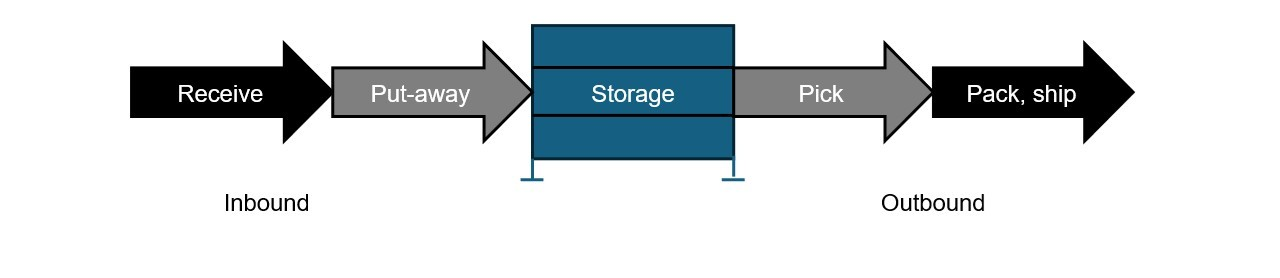
\includegraphics[width=0.95\textwidth]{figures/WarehouseFlowcr.jpg}
    \caption{Overview of the warehouse goods flow.}
    \label{fig:warehouse_order_fulfilment}
\end{figure}


Warehousing is a broad discipline with its own terminology and operational practices. This thesis introduces only the concepts necessary to understand the experimental environment; a more comprehensive discussion of warehouse operations can be found in Bartholdi and Hackman~\cite{bartholdi2019warehouse}.

In a typical warehouse, products are stored in designated storage locations such as shelves, racks, bins, or movable storage units. Customer requests are represented as orders that specify which items must be retrieved. The process of retrieving requested items from storage is commonly referred to as picking. Depending on the warehouse design, picked items may be transported to packing stations, where orders are prepared for shipment, before being sent to delivery or dispatch stations for onward transportation~\cite{bartholdi2019warehouse,dekoster2007design}.
\begin{figure}[H]
    \centering
    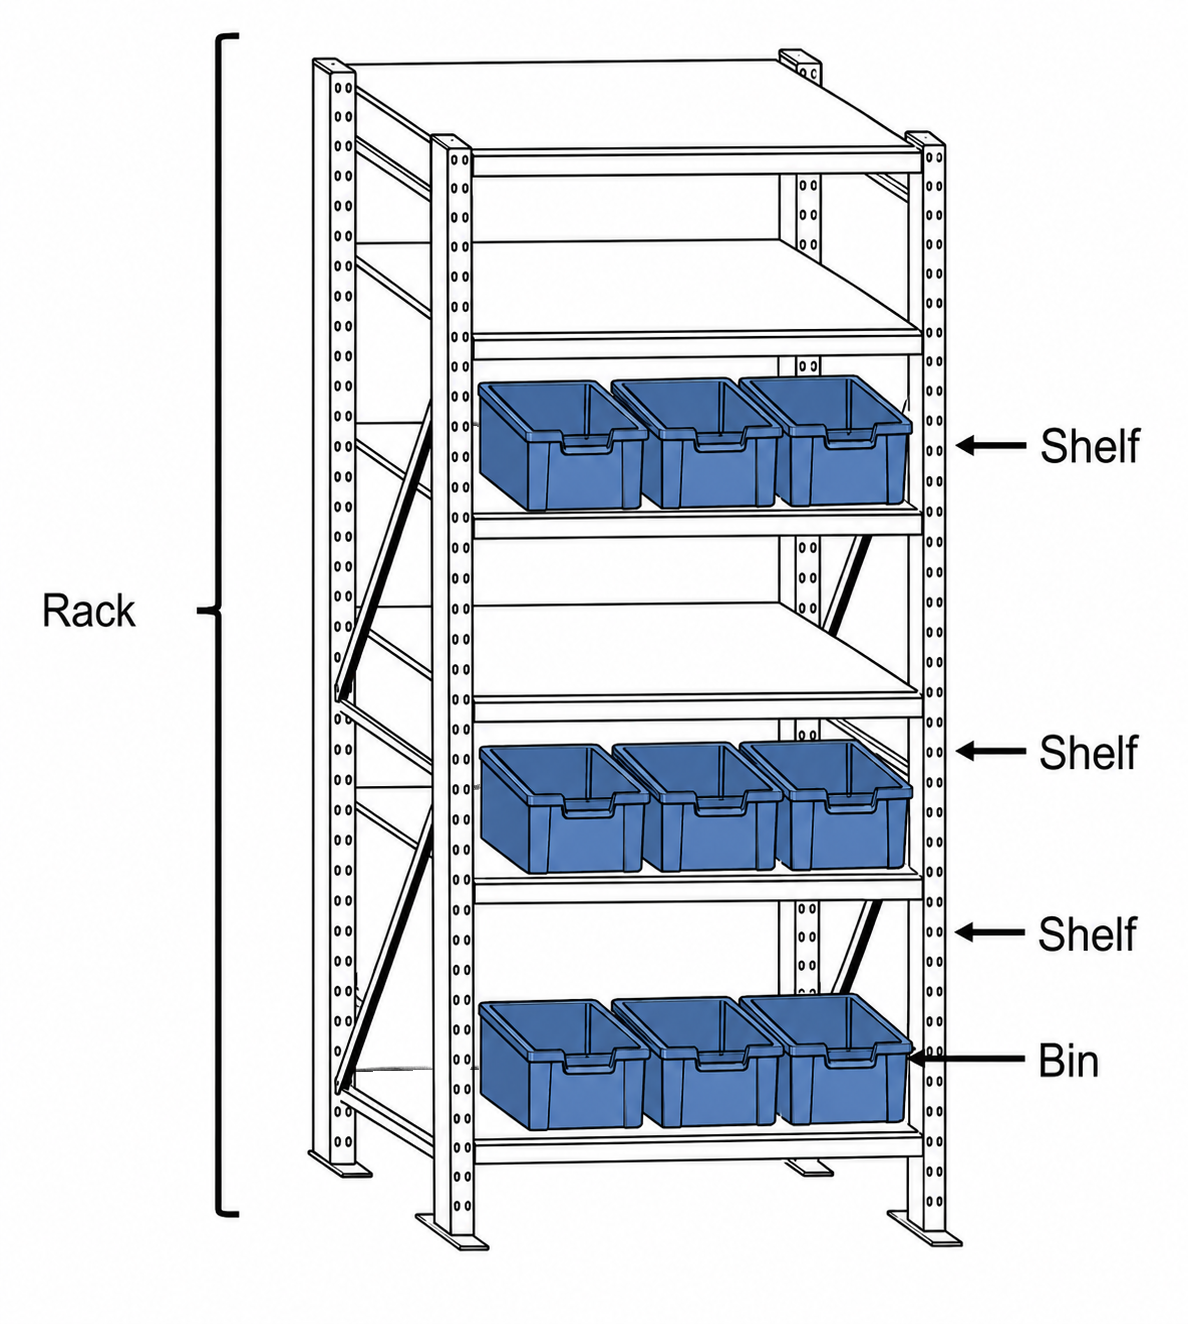
\includegraphics[width=0.95\textwidth]{figures/Rack-shelves-bin.png}
    \caption{Example warehouse storage hierarchy showing a rack composed of multiple shelves and storage bins.}
    \label{fig:warehouse_storage_hierarchy}
\end{figure}
The resources involved in these activities may include human workers, automated storage systems, mobile robots, workstations, and warehouse management software. Together, these components form a workflow whose objective is to fulfil customer orders accurately and efficiently.
Traditionally, warehouses operated according to a person-to-goods paradigm. Human workers travelled through storage aisles to locate and retrieve products. While straightforward to implement, worker travel often represented a significant portion of fulfilment time and operational cost~\cite{dekoster2007design}.

As order volumes increased, particularly with the growth of e-commerce, alternative approaches emerged. In goods-to-person systems, products or storage units are brought to stationary workers instead of requiring workers to travel throughout the warehouse. This reduces travel time but introduces new coordination challenges, since storage units, workstations, and transportation resources must now be scheduled and synchronised effectively~\cite{boysen2019warehousing,barros2021rmfs}.

Robotic warehouse systems emerged as a natural extension of this evolution.
A well-known example is the Kiva-style warehouse system, in which fleets of mobile robots transport inventory pods between storage areas and stationary workstations~\cite{wurman2008coordinating}. 
Unlike traditional racks, which remain fixed in place, inventory pods are movable storage units containing multiple shelves and stored products. Mobile robots navigate beneath these pods, lift them, and transport them to workstations where items can be retrieved~\cite{wurman2008coordinating}.

\begin{figure}[H]
\centering
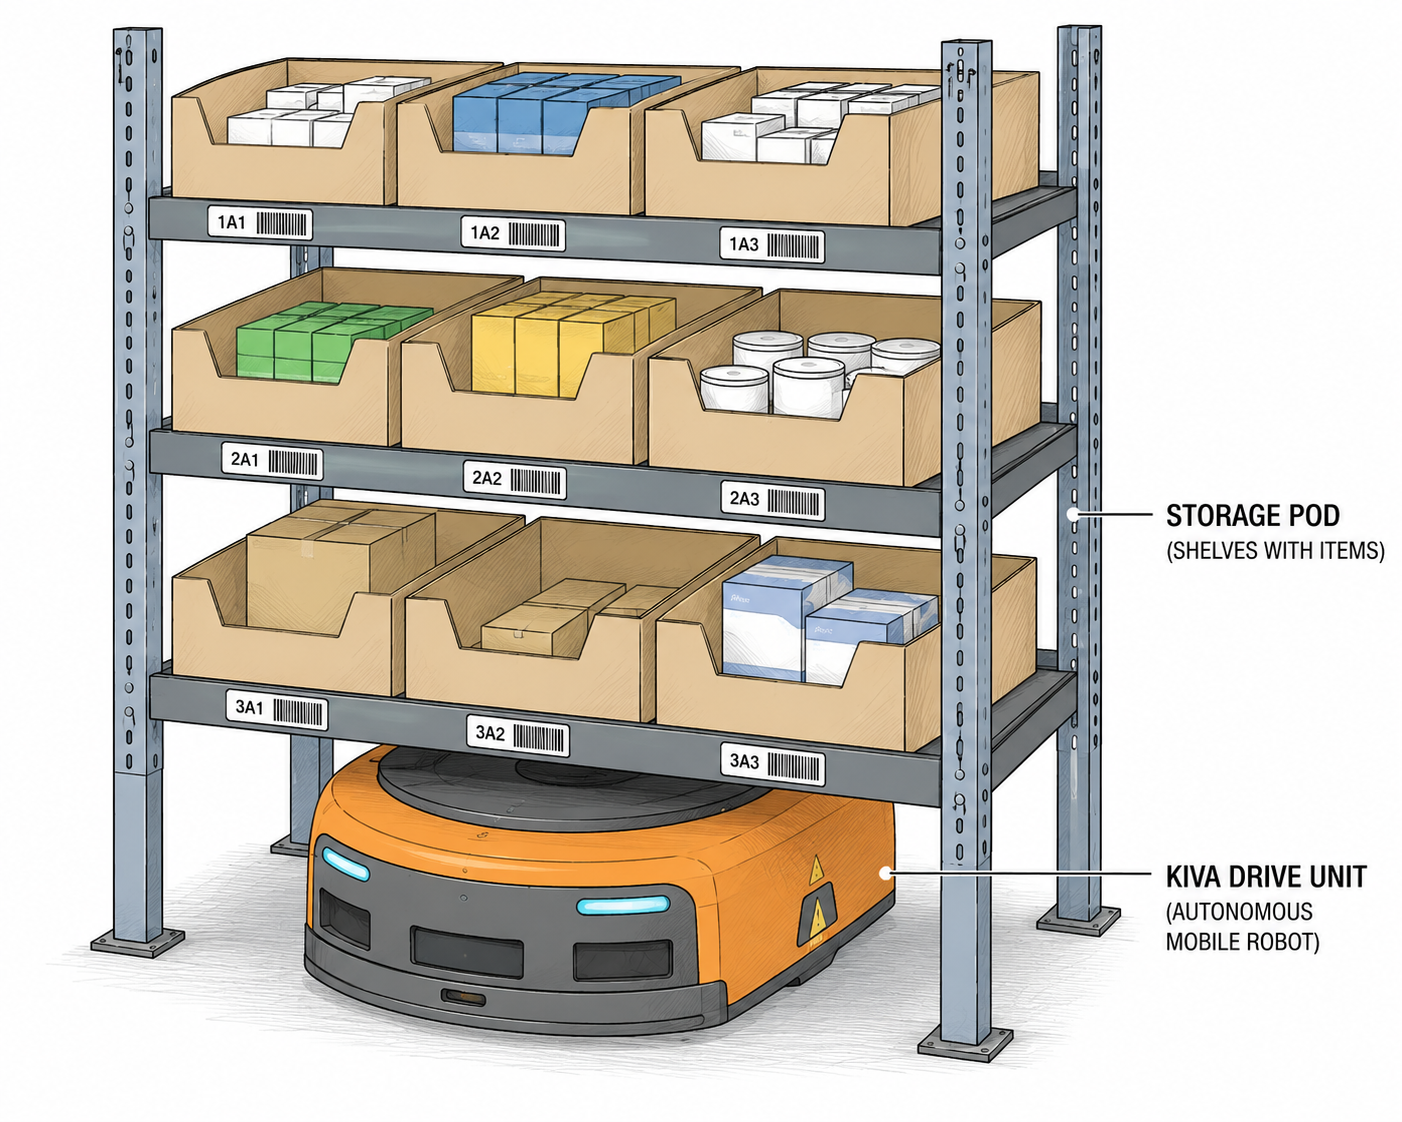
\includegraphics[width=0.95\textwidth]{figures/KivaWarehouse.png}
\caption{Illustration of a Kiva-style inventory pod. The pod contains multiple shelves used for product storage, while a mobile drive unit operates beneath the pod to transport it throughout the warehouse~\cite{wurman2008coordinating}.}
\label{fig:kiva_inventory_pod}
\end{figure}
Rather than asking workers to travel to products, the warehouse brings products to workers. By transporting storage units to stationary workstations, goods-to-person (GTP) systems reduce the need for worker travel and can improve fulfilment efficiency~\cite{wurman2008coordinating}. At the same time, they introduce additional coordination requirements among robots, storage units, and workstations.
The challenge is no longer limited to locating products and fulfilling orders. The warehouse must now determine which storage unit should be moved, which robot should perform the movement, which workstation should receive the requested items, and how shared resources should be allocated when multiple requests compete for attention. As the number of robots, workstations, and orders increases, these decisions become increasingly interdependent~\cite{wurman2008coordinating,barros2021rmfs}.

At this point, warehouse operation becomes a coordination problem. Robots may compete for pathways, storage units, charging stations, or workstations. Tasks may depend on the completion of other tasks. Some activities can be performed independently, while others require multiple resources or specialised roles to interact successfully. The overall performance of the warehouse depends on the capabilities of individual agents and the effectiveness of their coordination~\cite{yan2013mrscoordination}.
Although warehouse logistics provides a useful example, similar challenges appear throughout multi-agent systems. Autonomous vehicle fleets, drone swarms, manufacturing systems, search-and-rescue teams, and service robots must all operate under shared constraints while pursuing common objectives. The underlying challenge is therefore more general than warehouse automation: how can multiple agents make effective decisions while acting within a shared environment?

While coordination is essential in robotic warehouses, many real-world multi-agent systems require a stronger form of interaction. Coordination may be sufficient when agents perform largely independent tasks while sharing resources. Collaboration, however, requires agents to depend on one another in order to achieve a common objective. In such settings, successful task completion depends on the interaction of agents with complementary roles or capabilities~\cite{yan2013mrscoordination,karam2026collaborationmrs}.

Collaborative decision-making introduces additional challenges. Decisions made by one agent may influence the opportunities available to others, while task completion may depend on actions performed by multiple agents. Effective behaviour therefore requires consideration of shared goals, task dependencies, resource constraints, and the expected behaviour of teammates~\cite{karam2026collaborationmrs}. These characteristics make collaborative multi-agent systems an interesting domain for investigating whether language-model-based planning and decision-making can provide useful support.

In many practical multi-agent systems, this interdependence arises because agents possess complementary capabilities rather than identical roles. Progress may therefore depend on interactions between specialised agents that must work together to complete tasks.

Evaluating such decision-making approaches directly in physical robotic systems can be costly, difficult to reproduce, and potentially disruptive to ongoing operations. Changes to coordination or collaboration strategies may affect safety, productivity, equipment utilisation, and interactions between agents operating within the environment. Consequently, simulation has become a widely adopted methodology for studying multi-agent and multi-robot systems~\cite{papoudakis2021benchmarking,krnjaic2024warehouse}.


Simulation environments provide controlled and repeatable conditions in which task distributions, agent capabilities, resource constraints, and environmental characteristics can be varied systematically. This enables researchers to compare different approaches under identical conditions before considering deployment in physical systems.


The growing adoption of simulation has led to the development of standardised benchmark environments. Frameworks such as OpenAI Gym and its successor Gymnasium provide common interfaces that support reproducible experimentation across a wide range of reinforcement-learning and decision-making problems~\cite{brockman2016gym,towers2024gymnasium}.
Warehouse-inspired benchmark environments have become particularly popular because they capture many of the coordination and collaboration challenges encountered in real-world systems. Agents must share resources, resolve conflicts, allocate tasks, and operate towards common objectives while acting under environmental constraints. Although simplified relative to real warehouses, such environments provide a useful platform for studying multi-agent decision-making~\cite{krnjaic2024warehouse}.


Many approaches have been proposed for decision-making in multi-agent and multi-robot systems. Depending on the application, researchers have employed optimisation methods, heuristic approaches, rule-based control, task-allocation algorithms, and more recently multi-agent reinforcement learning. These techniques have demonstrated success across a variety of coordination and planning problems, but they may require domain-specific design, extensive training, reward engineering, or adaptation when objectives and environmental conditions change~\cite{gerkey2004formal,sharon2015conflict,papoudakis2021benchmarking}.


Recent advances in large language models have motivated interest in their use beyond traditional text-generation tasks. Their demonstrated ability to generate plans, reason about constraints, decompose tasks, and interpret structured descriptions of environments has led researchers to explore their use in planning and robotics applications~\cite{huang2022lmp,ahn2022do,liang2022code}. These developments raise the possibility that language models could serve as high-level decision-making components in collaborative multi-agent systems.

Despite growing interest in language-model-based planning, relatively little work has investigated their use for collaborative decision-making among heterogeneous agents operating under shared constraints. Existing studies often focus on single-agent tasks, embodied planning for individual robots, or coordination settings in which agents perform largely independent activities~\cite{huang2022lmp,ahn2022do,mandi2024roco}. Less attention has been given to environments where successful task completion depends on interactions between specialised roles and where decisions must remain grounded in a constrained action space.


Several practical questions therefore remain open. How does collaborative performance vary among locally deployable language models spanning different parameter scales? How should planning responsibilities be distributed when multiple agents require decisions? Does the representation used to describe the environment influence the quality of the resulting decisions? Addressing these questions is important for understanding whether language models can contribute to collaborative multi-agent systems and how such systems should be designed and deployed in practice.


To investigate these questions, the present thesis evaluates language models as high-level decision-making components within a collaborative multi-agent setting. Rather than focusing on low-level robot control, the study examines how different design choices influence collaborative task performance. In particular, three factors are considered: model choice across nominal parameter scales, the architecture used for planning, and the representation used to describe the environment state.

One important design consideration concerns the planning architecture. In a \emph{centralized planning} approach, a single prompt receives a shared description of the environment and returns decisions for all agents requiring planning. An alternative approach is \emph{shared-context per-agent planning}, where agents are planned individually but each prompt still contains a summary of the shared environment state. These approaches represent different ways of distributing decision-making responsibility while maintaining access to global context.

Another important consideration concerns how information is presented to the language model. Software and robotic systems commonly exchange information using structured data representations rather than natural language. One widely adopted format is JavaScript Object Notation (\gls{json}), which represents system state through structured key-value pairs and hierarchical data structures. Such representations are convenient for software integration because they can often be generated directly from program variables with minimal transformation.

However, language models are primarily trained on human-generated text and may therefore process information differently depending on how information is represented. Recent studies suggest that prompt structure and information representation can influence language-model behaviour and task performance, while structured formats may affect reasoning performance in some settings~\cite{sahoo2024promptsurvey,tam2024letmespeak}. This creates an important practical question for engineering applications. Should system state be provided directly in a structured format such as \gls{json}, or is it beneficial to invest additional effort in transforming the same information into natural-language descriptions that more closely resemble the data on which language models were trained? The present thesis investigates this question alongside model choice across parameter scales and planning architecture.
\subsection{Research Questions}
\label{sec:rq}
The thesis is guided by the following main research question:

\begin{quote}
\textbf{Main Research Question:} Can prompted \glspl{llm} support grounded high-level decision-making for heterogeneous multi-robot collaboration in a constrained warehouse environment?
\end{quote}

To investigate this question systematically, the study examines three design factors: model choice across nominal parameter scales, planning architecture, and prompt configuration. The following sub-questions are considered:

\begin{enumerate}
\item \textbf{RQ1 (Model Choice Across Parameter Scales):} How does grounded collaborative task performance vary among selected locally deployable language models spanning different nominal parameter sizes?

\item \textbf{RQ2 (Planning Architecture):} How do centralized planning and shared-context per-agent planning differ in their ability to support collaborative task performance across scenarios with varying collaboration demands?

\item \textbf{RQ3 (Prompt Configuration):} How does collaborative task performance differ between the tested natural-language and \gls{json}-based prompt configurations?
\end{enumerate}

The research questions are evaluated in a warehouse-inspired collaborative environment involving heterogeneous agents operating under shared constraints. Performance is assessed using delivery count, model-interaction frequency, and behaviour across scenario configurations. Generation and action-validation failures are retained as diagnostic fields for run validation rather than treated as separate research outcomes.

\subsection{Contributions}
\label{sec:contrib}

This thesis contributes:

\begin{itemize}
\item A grounded evaluation framework for studying language-model-based high-level decision-making in collaborative heterogeneous multi-robot systems. The approach constrains language-model outputs to environment-defined actions and validates proposed decisions against explicit feasibility constraints.

\item Comparative empirical observations across selected models spanning different parameter scales, planning architectures, and prompt configurations in language-model-based collaborative decision-making. The results characterise differences in delivery performance and language-model utilisation under the grounded control interface.
\end{itemize}


\subsection{Report Outline}
Section~\ref{sec:background} provides background on multi-robot coordination, warehouse task assignment, and \gls{llm}-based planning.
Section~\ref{sec:method} describes the environment, the proposed \gls{llm} control loop, the experimental design, and the main delimitations of the study.
Section~\ref{sec:result_discussion} presents the experimental results together with their interpretation.
Section~\ref{sec:ethics_sustainability} discusses ethical and sustainability considerations.
Finally, Section~\ref{sec:conclusions} concludes the thesis and outlines future work.


\section{Background and Related Work}
\label{sec:background}
This chapter reviews the literature relevant to language-model-based task planning in heterogeneous multi-robot systems. It examines the evolution of task planning approaches, recent advances in language-model-based planning, grounding and environment representation, language model selection, and simulation environments. Together, these developments establish the current state of the field and motivate the research presented in this thesis.

Task planning is a fundamental problem in multi-robot systems, concerned with allocating, ordering, and coordinating tasks among multiple robots to achieve a shared objective efficiently. Unlike single-robot planning, multi-robot systems must additionally consider interactions between agents, including resource sharing, communication, task dependencies, and conflicting objectives. As the number of robots and the complexity of the environment increase, the planning problem becomes increasingly difficult due to the combinatorial growth of possible task allocations and execution sequences.

Early research addressed these challenges using explicitly engineered planning and coordination strategies based on optimisation, heuristics, and predefined decision rules. Gerkey and Matari\'c~\cite{gerkey2004formal} formalised the Multi-Robot Task Allocation (MRTA) problem and proposed a taxonomy for categorising task allocation methods according to robot capabilities, task characteristics, and allocation strategies. Their work established a common framework for analysing and comparing multi-robot planning algorithms and continues to influence subsequent research.

Yan \textit{et al.}~\cite{yan2013mrscoordination} subsequently reviewed the broader field of multi-robot coordination, covering auction-based task allocation, cooperative transport, communication-aware coordination, motion planning, and early learning-based methods. Representative systems such as MURDOCH demonstrated that distributed auction mechanisms could efficiently allocate tasks among heterogeneous robots, while other approaches incorporated temporal dependencies, spatial constraints, and robot availability during cooperative task execution. These studies showed that successful multi-robot task planning depends on task allocation, communication, coordination, synchronisation, and conflict resolution.

Although heuristic and optimisation-based approaches proved effective in structured environments, they relied heavily on handcrafted rules, explicit environment models, and manually designed objective functions. Adapting these systems to new environments or operational requirements often required substantial redesign, which encouraged increasing interest in learning-based approaches.

Learning-based planning, particularly Reinforcement Learning (RL) and Multi-Agent Reinforcement Learning (MARL), enables robots to learn coordination policies through repeated interaction with the environment instead of relying on predefined decision rules. Compared with classical planning methods, MARL offers greater adaptability to dynamic environments by allowing cooperative behaviours to emerge through experience. It has therefore become a prominent approach for heterogeneous multi-robot coordination.

Papoudakis \textit{et al.}~\cite{papoudakis2021benchmarking} addressed the lack of standardised evaluation in MARL by comparing representative independent learning, policy-gradient, and value-decomposition algorithms across a diverse collection of cooperative tasks. Their study showed that algorithm performance depends strongly on task characteristics such as reward sparsity and coordination complexity while introducing the EPyMARL framework and additional benchmark environments to support reproducible evaluation.

Later work by Krnjaic \textit{et al.}~\cite{krnjaic2024warehouse} applied hierarchical MARL to heterogeneous warehouse logistics involving autonomous mobile robots and human workers. Their manager-worker architecture decomposed decision making into hierarchical levels, improving sample efficiency and warehouse throughput compared with conventional MARL methods and industrial heuristic approaches. The authors also introduced the Task Assignment Robotic Warehouse (TA-RWARE) benchmark, extending RWARE to support heterogeneous task allocation and providing a reproducible platform for evaluating high-level coordination strategies.

Subsequent research shifted attention towards improving cooperation through reward design. Niu and Gürdür Broo~\cite{niu2025rewardshaping} proposed a biologically inspired reward shaping framework based on ecological symbiosis, demonstrating improved convergence stability and cooperative behaviour in heterogeneous robotic systems. Niu \textit{et al.}~\cite{niu2025symbiosis} later incorporated symbiotic principles into a Centralised Training with Decentralised Execution (CTDE) MARL framework, enabling robots to coordinate battery management and workload distribution through shared state information. Their results demonstrated improvements in task performance, resource utilisation, and energy management in simulated warehouse environments.

Despite these advances, learning-based approaches remain dependent on environment-specific training, carefully designed reward functions, and computationally intensive policy optimisation. Adapting trained policies to new environments or task configurations often requires additional training or redesign. These limitations have led researchers to investigate pretrained Large Language Models (LLMs) as an alternative paradigm for high-level task planning, seeking to exploit the reasoning capabilities acquired during large-scale pretraining instead of learning task-specific policies from scratch.

Li et al.~\cite{li2026largelanguagemodelsmultirobot} classify LLM applications in robotics according to the level of decision making they support, including high-level task planning and task allocation, mid-level motion planning, and low-level action generation. High-level planning concerns reasoning over task objectives and coordination, whereas lower levels focus on trajectory generation or direct robot control.

Existing LLM-based planning frameworks commonly employ language models as high-level decision makers while retaining conventional perception, navigation, and control modules. SayCan grounds language-model action selection with affordance estimates so that plans are biased towards actions that are both useful for the instruction and feasible in the current robotic state~\cite{ahn2022do}. Inner Monologue extends this pattern by incorporating feedback from the environment into language-model planning, while ProgPrompt represents situated task plans as program-like structures over available robot actions~\cite{huang2022innermonologue,singh2023progprompt}. Code as Policies instead uses the language model to generate executable programs over predefined robot APIs, making code the intermediate policy representation between language instructions and embodied control~\cite{liang2022code}. Related zero-shot planning work shows that language models can propose action sequences from textual task descriptions when they are given an explicit action interface, although such plans still require grounding, validation, and replanning when deployed in physical or simulated environments~\cite{huang2022lmp}.

Extending \glspl{llm} from single-robot planning to multi-robot systems introduces additional challenges related to communication, coordination, and information sharing among multiple autonomous agents. Unlike single-robot systems, where a single planning context is sufficient, multi-robot systems must determine how planning responsibilities and information should be distributed across multiple agents. Consequently, recent research has explored a range of planning and communication architectures for integrating \glspl{llm} into collaborative multi-robot systems~\cite{li2026largelanguagemodelsmultirobot}.

One line of research investigates how individual language models should be orchestrated across multiple agents. Liu \textit{et al.}~\cite{liu2023bolaa} analysed several architectures for LLM-augmented autonomous agents, ranging from simple zero-shot planning to iterative self-reflection frameworks that incorporate previous observations and actions into subsequent reasoning steps. Their work also proposed BOLAA, an orchestration strategy in which a controller manages communication among multiple specialised language-model agents. Although their study primarily considers general autonomous-agent benchmarks rather than physical robot teams, the proposed orchestration strategies provide useful insights for multi-robot coordination.

In robotics, Mandi \textit{et al.}~\cite{mandi2024roco} proposed RoCo, a multi-robot collaboration framework in which language-model agents discuss task strategies, generate sub-task plans, and revise plans using feedback such as collision checking. This work demonstrates how dialogue and shared feedback can be used to coordinate multiple robots, but it also illustrates the need for explicit grounding and validation when language models are used inside embodied planning loops.

Although \glspl{llm} possess extensive world knowledge acquired during pretraining, they do not have direct knowledge of the robot's current environment. Consequently, generated plans may reference unavailable objects, infeasible actions, or incorrect assumptions about the world state, a phenomenon commonly referred to as hallucination. Grounding addresses this problem by constraining language-model reasoning using information obtained from the environment, ensuring that generated plans remain both logically and operationally feasible.

Existing work has explored several approaches for grounding LLMs in robotic task planning. SayCan constrains language-model reasoning through affordance-based action selection, ensuring that generated actions are executable in the current environment~\cite{ahn2022do}. Feedback-based approaches further improve planning reliability by incorporating observations from the environment during execution, allowing the language model to identify infeasible plans and refine subsequent decisions through iterative replanning~\cite{huang2022innermonologue,bhat2025closedloopgrounding}. Recent surveys identify grounding as a fundamental requirement for improving the robustness and reliability of LLM-based robotic planning systems~\cite{li2026largelanguagemodelsmultirobot}.

Regardless of the grounding mechanism employed, the language model ultimately reasons over an abstract representation of the environment describing the available objects, actions, and current system state. Existing work has represented this information using natural-language descriptions, symbolic planning languages, executable code, and other structured representations. The choice of representation influences both the information available to the language model and the ease with which generated plans can be validated and executed, making environment representation an important design consideration for LLM-based task planning.

Structured representations such as JSON have become increasingly common in LLM-based planning because they encode hierarchical information through key-value pairs while remaining machine-readable and readily integrated with existing robotic software. In contrast, natural-language descriptions provide greater flexibility in expressing task context and relationships between entities. Consequently, both structured and natural-language representations have been adopted for conveying environment state to language models. However, recent work suggests that imposing restrictive formats may also influence language-model reasoning. Tam \textit{et al.}~\cite{tam2024letmespeak} showed that strict output format constraints can reduce LLM performance on reasoning tasks, highlighting a potential trade-off between structured representations and generation flexibility. Despite the increasing use of both approaches, their impact on high-level task planning performance in heterogeneous multi-robot systems remains insufficiently understood.


Language model selection represents another important design consideration in LLM-based robotic planning. In applied robotics and embedded systems, constraints on computation, memory, energy consumption, and inference latency may favour the deployment of smaller language models over larger alternatives~\cite{dawane2026onddeviceslm}. However, smaller models often exhibit weaker reasoning capabilities and may therefore require more carefully designed prompts, structured task representations, or additional validation mechanisms to achieve reliable planning performance.Xiao et al. and Mandi et al.~\cite{xiao2026probingprompt,mandi2024roco} investigated prompt design as a means of compensating for limited model capacity and improving decision quality in resource-constrained deployments. At the same time, studies have shown that imposing restrictive prompt or output formats may negatively influence language-model reasoning, suggesting a trade-off between structured machine-readable representations and generation flexibility~\cite{sahoo2024promptsurvey,tam2024letmespeak}. Collectively, these studies indicate that planning performance depends not only on the choice of language model, but also on how planning problems are represented and communicated to the model.

A variety of simulation environments have been developed to evaluate multi-robot planning and coordination algorithms. These include warehouse-specific benchmarks, industrial warehouse simulators, and general-purpose robotic simulation platforms such as NVIDIA Isaac Sim, with the choice of simulator typically depending on the planning problem under investigation~\cite{krnjaic2024warehouse,niu2025symbiosis}.

Among warehouse-specific benchmarks, the Multi-Robot Warehouse (RWARE) environment introduced by Papoudakis \textit{et al.}~\cite{papoudakis2021benchmarking} models a partially observable grid-world warehouse in which multiple robots cooperate to retrieve requested shelves and deliver them to workstations. Agents receive sparse rewards only after successfully completing a sequence of coordinated actions, making coordination difficult and providing a challenging benchmark for cooperative multi-agent reinforcement learning.

To investigate heterogeneous task allocation, Krnjaic \textit{et al.}~\cite{krnjaic2024warehouse} extended RWARE to develop the Task-Assignment Robotic Warehouse (TA-RWARE) environment. TA-RWARE introduces two heterogeneous agent roles, Automated Guided Vehicles (AGVs) and picker robots, which cooperate to complete warehouse operations. Instead of directly controlling robot motion, agents select target locations while navigation between locations is performed using a predefined path-planning heuristic. By abstracting low-level navigation, the environment enables researchers to focus on high-level task assignment and coordination in heterogeneous multi-robot systems.


\section{System and Method}
\label{sec:method}
\subsection{Overview}
This chapter serves two roles.
It describes the implemented system, but it also justifies the empirical design used to answer the research questions.
The thesis is therefore structured as a comparative experimental study: the same warehouse environment, evaluation metrics, and scenario catalogue are reused while selected design variables are changed in order to study their effect on collaborative task performance.

This design is appropriate for the thesis because the research questions are comparative rather than purely descriptive.
RQ1 asks how model size affects performance, RQ2 asks how planning architecture affects performance, and RQ3 asks how prompt representation affects performance.
These questions require the report to make explicit what is fixed, what is varied, and how the experiments are structured across the objective families.

The thesis uses an empirical, experimental methodology:
\begin{enumerate}
    \item Implement an \gls{llm}-driven control loop for a simulated heterogeneous warehouse environment.
    \item Define the main comparison axes and evaluation metrics.
    \item Run controlled experiments (fixed environment ids and seeds) across multiple \gls{llm} models, planning architectures, and prompt variants.
    \item Analyze throughput, safety, and collaborative task outcomes as well as qualitative failure modes.
\end{enumerate}

\paragraph{What is fixed and what is varied.}
Across the main experiment families, the environment, action space, scenario catalogue, evaluation metrics, grounding/validation scheme, and local-inference setup are held as stable as practical.
The principal variables are model size, planning architecture, prompt representation, and objective family.
The report does not use an external heuristic baseline in the current comparison set, so the reported comparisons are made within the language-model-based control framework.

\paragraph{Interpretation and controls.}
The experiments are controlled in the sense that scenario ids, seeds, and runner configurations are recorded and reused within each family.
The surrounding validation layer filters infeasible outputs before execution, and the same comparison axes are used across the objective families.

\subsection{Environment: Battery-TA-RWARE}
Battery-TA-RWARE is a discrete-time, grid-based warehouse simulation derived from \gls{tarware}~\cite{krnjaic2024warehouse}.
At any time, a set of shelves is requested. Carrier \glspl{agv} must transport requested shelves to goal locations and then return them to storage.
Picker agents are required to meet \glspl{agv} at shelf locations for load and unload interactions, creating explicit heterogeneous coordination constraints.
Agents additionally have a battery state that decreases with movement and interactions; charging stations are available at fixed locations.

\begin{figure}[H]
    \centering
    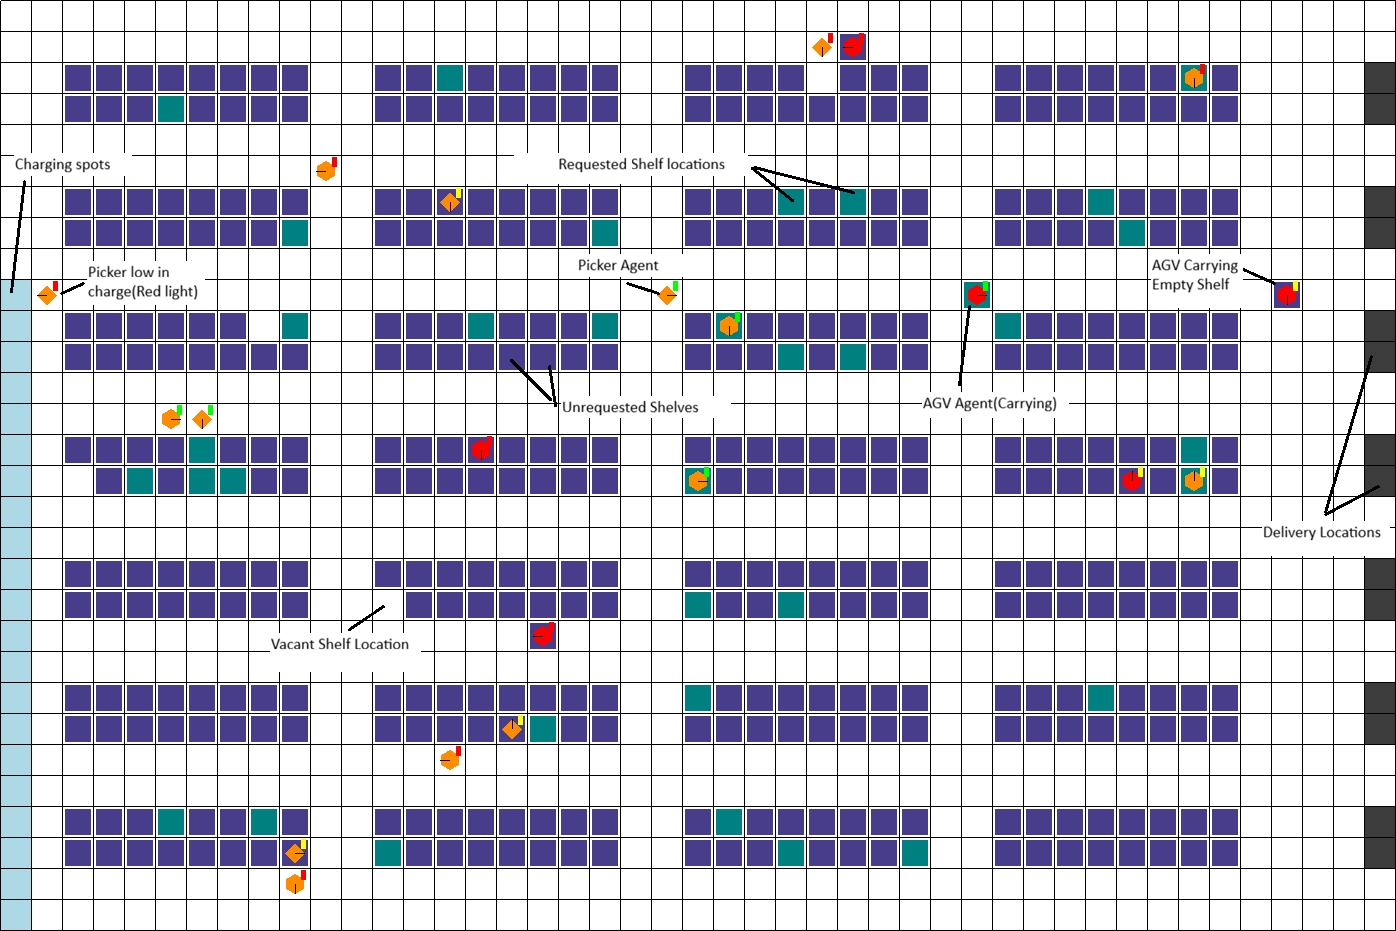
\includegraphics[width=0.95\textwidth]{../Battery-TA-RWARE/docs/img/BatteryTA-RWARE.png}
    \caption{Illustration of the task-assignment warehouse setting used in this thesis.}
    \label{fig:tarware_overview}
\end{figure}

The environment exposes a discrete action space where each action corresponds to selecting a target location:
\begin{itemize}
    \item \textbf{Shelf actions:} choose a shelf location (e.g., to pick up or return a shelf).
    \item \textbf{Goal actions:} choose a delivery station (primarily relevant when an \gls{agv} carries a requested shelf).
    \item \textbf{Charging actions:} choose a charging station to recover battery.
\end{itemize}
Low-level motion toward the selected target is handled internally by the environment (A* path planning and collision resolution), while the controller is evaluated on the quality of these high-level decisions.

\subsection{Language-Model Control Loop}
\label{sec:llm_loop}
The \gls{llm} policy is implemented as a text-in / discrete-action-out controller:
\begin{enumerate}
    \item \textbf{State summarization:} extract salient features of the global state (requested shelves and their action ids, per-agent position/target/battery/carrying status, charging occupancy).
    \item \textbf{Candidate action set:} compute a valid-action mask from the environment and derive the prompt-visible candidate set from those feasible actions. These candidates are presented as compact role-relevant action rows with action ids and guidance fields such as distance, tags, and charging-related instructions.
    \item \textbf{Prompting:} generate a per-agent prompt describing the agent role and the current state, including explicit mappings from requested objects to action ids.
    \item \textbf{Querying:} send the prompt to a local inference server (Ollama) and obtain a text response.
    \item \textbf{Parsing:} parse an integer action id (and optionally an action hold duration) from the response.
    \item \textbf{Validation:} validate the parsed action id against the current valid-action mask. If the proposed action is missing or invalid, the controller discards it and falls back to an idle action for that step; in the action-persistence setting, an invalid persisted action clears the hold and forces a new query.
    \item \textbf{Execution:} apply the validated joint action in the environment for one step (or hold the action for multiple steps, depending on configuration).
\end{enumerate}

\begin{figure}[H]
    \centering
    \begin{tikzpicture}[
        node distance=5mm,
        box/.style={draw, rounded corners, align=center, minimum width=0.7\textwidth, minimum height=8mm},
        arrow/.style={-Latex, thick}
    ]
        \node[box] (state) {State summary from the current environment step};
        \node[box, below=of state] (candidates) {Candidate shaping and feasible-action mask};
        \node[box, below=of candidates] (prompt) {Prompt construction for joint or per-agent planning};
        \node[box, below=of prompt] (query) {Language-model query};
        \node[box, below=of query] (parse) {Parse action identifier and optional hold duration};
        \node[box, below=of parse] (validate) {Validate against current constraints};
        \node[box, below=of validate] (execute) {Execute one environment step or continue a persisted action};
        \node[box, below=of execute] (feedback) {Observe step consequence and decide whether replanning is needed};
        \draw[arrow] (state) -- (candidates);
        \draw[arrow] (candidates) -- (prompt);
        \draw[arrow] (prompt) -- (query);
        \draw[arrow] (query) -- (parse);
        \draw[arrow] (parse) -- (validate);
        \draw[arrow] (validate) -- (execute);
        \draw[arrow] (execute) -- (feedback);
        \draw[arrow] (feedback.east) -- ++(2.2,0) |- (state.east);
    \end{tikzpicture}
    \caption{Schematic of the language-model control loop used in the experiments.}
    \label{fig:lm_control_loop}
\end{figure}

The controller is best described as a discrete-time, step-synchronous supervisory loop with conditional replanning.
The environment advances one simulation step at a time, and at each step the controller reevaluates agent state and action validity.
However, this does not imply that every agent is queried at every step.
Instead, the experiments use two related control schemes.

\begin{itemize}
    \item \textbf{Step-synchronous replanning with environment-owned continuation:} agents that are currently available for planning may receive a new high-level action, while busy agents are not replanned and continue their current task until the environment releases them.
    \item \textbf{Step-synchronous replanning with action persistence and conditional override:} accepted actions may remain active for multiple future steps, so agents are not re-queried while the persisted action remains valid. Replanning is triggered when a persisted action expires, becomes invalid, or when the controller decides intervention is needed, including selected busy-agent cases.
\end{itemize}

This design sits between two extremes.
A fully scheduled scheme that queries every agent at every step would generate many unnecessary \gls{llm} calls, while a purely event-triggered scheme is less natural in this setting because useful triggers such as blocked progress, invalid persisted actions, expiring commitments, or changing support needs are only known after the system state is checked.
The adopted design therefore combines regular per-step observability with selective replanning.
This is also consistent with practical supervisory control in warehouse systems, where the fleet is typically checked at regular intervals, ongoing tasks continue by default, and new task-level decisions are issued only when the current situation justifies intervention.

Two design choices are central for feasibility:
\begin{itemize}
    \item \textbf{Grounding via action ids:} the \gls{llm} does not output coordinates or free-form text commands; instead it selects from discrete action ids that are already defined by the environment.
    \item \textbf{Hard validation:} action masks enforce constraints such as invalid goals for picker agents and busy-state restrictions. Invalid \gls{llm} outputs are never executed.
\end{itemize}

The reported behaviour is therefore the behaviour of the complete control framework: prompt design, model output, candidate shaping, validation logic, and replanning policy act together inside the same supervisory loop.

\subsection{Experiment Design and Comparison Axes}
The experiments are organized as a controlled comparison within the grounded language-model control loop described above.
Across the experiment families, the environment, discrete action space, validation layer, scenario catalogue, local-inference setup, and evaluation metrics are kept as stable as practical.
The main factors that change are the objective formulation, model size, planning architecture, and prompt representation.
This structure is important because the thesis does not only ask whether an \gls{llm} can control the warehouse agents; it asks how different ways of using the \gls{llm} affect collaborative task performance under comparable conditions.

The objective families define the main progression of the experimental campaign.
The first family uses a delivery-only objective, where the controller is evaluated primarily on raw shelf-delivery throughput.
This establishes the baseline interpretation for the later experiments: the controller is expected to select high-level actions that move requested shelves through the warehouse as effectively as possible.
The second family keeps the same warehouse task and comparison axes, but changes the objective into a call-aware formulation that seeks to maintain delivery performance while reducing unnecessary \gls{llm} queries.
In this family, the output interface includes a \nolinkurl{Steps} field, allowing a selected action to persist for multiple simulation steps when repeated replanning is not useful.
The third family extends the same framework toward battery-aware control, where the purpose is to study whether the controller can incorporate resource constraints in addition to throughput and call efficiency.
Together, these objective families make it possible to compare not only absolute delivery performance, but also how the same supervisory loop behaves when the definition of a good decision changes.

Two planning architectures are compared inside this framework.
In the centralized architecture, one \gls{llm} call plans for all agents that currently need a decision, using a prompt that exposes the global state and the relevant candidate actions.
This gives the model an explicit opportunity to coordinate joint behaviour, but it also increases the prompt size and output complexity as the number of agents and candidate actions grows.
In the shared-context per-agent architecture, the model plans for one agent at a time.
Each prompt still contains global information, but the required output concerns only the current agent.
This reduces parsing burden and makes the decision format simpler, while shifting coordination from one explicit joint plan to a sequence of local decisions made with shared context.
The comparison is therefore meaningful because it separates two practical ways of embedding language models in multi-agent control: broad joint reasoning versus simpler repeated decisions.

Prompt representation is treated as another comparison axis rather than as a separate experiment in isolation.
The prompts always ground the model's choice in explicit action ids and role-relevant state, including requested-shelf mappings, rules for \glspl{agv} and pickers, support relations such as waiting-for-picker context, battery-state abstractions, and filtered or prioritized candidate actions.
What varies is the form in which the model is asked to respond, especially natural-language action selection versus structured \gls{json} output.
This comparison tests whether stronger output structure improves reliability without changing the underlying warehouse task.
Taken together, the principal comparison axes are model size, centralized versus shared-context per-agent planning, natural-language versus \gls{json} prompting, and the three objective formulations of delivery-only, call-aware delivery, and battery-aware control.

\subsection{Scenarios, Models, and Metrics}
The same scenario catalogue is reused across the experiment families so that differences in observed behaviour can be interpreted against known coordination pressures rather than against unrelated task changes.
The scenarios are \nolinkurl{tiny_balanced_1v1}, \nolinkurl{small_balanced_2v2}, \nolinkurl{medium_balanced_4v4}, \nolinkurl{small_agv_heavy_4v2}, \nolinkurl{medium_agv_heavy_6v2}, and \nolinkurl{small_picker_heavy_2v4}.
These scenarios cover simple balanced collaboration, increased concurrency, larger warehouse layouts, \gls{agv}-heavy settings where picker support can become a bottleneck, and picker-heavy settings where allocation efficiency and underutilization become more visible.
The scenario set therefore tests whether a model, prompt form, or planning architecture remains productive when the source of coordination difficulty changes.

The model set spans smaller and larger local models: \nolinkurl{llama3.2:1b}, \nolinkurl{llama3.2:3b}, \nolinkurl{mistral:7b}, \nolinkurl{gemma3:12b}, \nolinkurl{phi4}, and \nolinkurl{qwen2.5:14b}.
Using models of different sizes supports the thesis question about whether larger models produce better coordination, or whether smaller models can remain competitive when the prompt is sufficiently grounded and the validation layer prevents infeasible actions from being executed.
Because all models operate through the same discrete-action interface, the comparison concerns decision quality within the same controller framework rather than differences in low-level robot control.

The primary metric is delivery throughput, expressed as pick rate, which is computed from the number of delivered shelves and the simulated episode duration.
Total shelf deliveries are also reported directly because they are easy to interpret in relation to the task objective and the episode-level delivery ceiling.
Additional metrics are collected to explain how a controller reaches its throughput outcome: clashes, deadlocks or stuck events, distance travelled by each agent type, episode return, episode length, and inference speed or latency when measured.
These supporting metrics are necessary because two configurations can achieve similar delivery counts for different reasons.
For example, one configuration may maintain throughput with fewer model calls, while another may show the same delivery count but with more clashes, longer no-delivery tails, or inefficient movement.
The metrics therefore connect the numerical result to the underlying collaborative behaviour.

\subsection{Experimental Protocol}
The reported experiment sessions were run with fixed environment ids and a fixed seed, creating a controlled set of comparable runs for the reported objective families.
Within that controlled setup, the campaign proceeds from Objective~1 delivery-only experiments to Objective~2 call-aware delivery experiments and then to Objective~3 battery-aware experiments.
This ordering is deliberate.
The delivery-only experiments first establish how the models, prompt forms, and planning architectures behave when the objective is simply to complete warehouse deliveries.
The call-aware experiments then ask whether the same framework can reduce unnecessary replanning without losing the productive behaviour established in the first family.
The battery-aware experiments extend the evaluation to resource-sensitive decision making, where the controller must consider battery constraints as part of the same high-level assignment problem.

Section~\ref{sec:result_discussion} reports Objective~1 for the shelf-delivery comparisons, Objective~2 for the call-aware comparisons, and Objective~3 for the battery-aware objective.
In the current simulation setup, a run can achieve at most 20 deliveries, and the results chapter uses that ceiling to contextualize reported scores.

\subsection{Delimitations}
To keep the study focused and interpretable, the following delimitations apply:
\begin{itemize}
    \item The work is evaluated in a simulated warehouse environment rather than on physical robots.
    \item The controller is responsible only for high-level target selection; low-level navigation and collision handling are performed by the environment.
    \item The evaluated language models are prompted general-purpose models accessed through a local inference server and are not fine-tuned for this task.
    \item The reported experiments use fixed seeds and a limited number of completed sessions.
    \item Completed aggregate results are not yet available for the battery-aware objective family.
\end{itemize}

\subsection{Ethical and Sustainability Considerations}
Although the present work is simulation-based, it raises practical issues that remain relevant for real multi-robot deployments.
The primary ethical concern is safety and reliability: generated decisions may be infeasible, unstable, or unproductive if they are not constrained by system-side checks.
For that reason, the studied control loop does not execute free-form outputs directly. It uses grounded action identifiers, candidate shaping, explicit feasibility validation, and fallback behavior so that unsafe or clearly invalid actions are filtered before execution.
The logging of prompts, parsed outputs, executed actions, and observed step consequences also improves traceability, which is important when analyzing failures such as long no-delivery tails, stale waiting loops, or battery-related breakdowns.

From a sustainability perspective, the main trade-off is between model capability and computational cost.
Larger language models generally require more inference time and compute, while smaller models may require stronger prompt structure and validation to remain effective.
This thesis therefore treats call efficiency, unnecessary replanning, and coordination overhead as practically relevant concerns rather than only implementation details.
Even with safeguards, fixed-seed evaluation, limited scenario coverage, and the absence of physical deployment still bound the scope of the reported results.


\section{Preliminary Results and Discussion}
\label{sec:result_discussion}
\subsection{Experimental Data Overview}

The results are organised around the three research questions introduced in Section~\ref{sec:rq}. The analysis focuses on three main comparison axes: prompt configuration, planning architecture, and model behaviour across scenario configurations. In addition, an exploratory analysis is included for objective sensitivity.

The metrics and experimental conditions are defined in Section~\ref{sec:method_scenarios_models_metrics}. This chapter reports raw shelf deliveries and \gls{llm} calls together with the call-normalised delivery measure defined in Eq.~\ref{eq:deliveries-per-1000-calls}. Raw delivery count remains the main task-completion measure, while the call-normalised value describes deliveries relative to model-interaction frequency. The analyses use matched configuration-level observations drawn from the Calls, Battery + Shelf, and Battery objective families. Repeated executions with the same objective, architecture, prompt configuration, model, and scenario identifiers are averaged before matching, and therefore do not receive additional weight.

\subsection{RQ3: Prompt-Configuration Comparison}
\label{sec:results_prompt_representation}

RQ3 compares collaborative task performance under the tested natural-language and \gls{json}-based prompt configurations. Table~\ref{tab:json_natural_scenario} reports the scenario-level comparison, using 144 matched configuration-level observations for each prompt configuration. Across all six scenarios, the natural-language configuration produced higher mean deliveries and higher deliveries per 1000 calls than the \gls{json}-based configuration.

\begin{table}[H]
\centering
\small
\resizebox{\textwidth}{!}{%
\begin{tabular}{|l|c|c|c|c|}
\hline
\textbf{Scenario} & \textbf{JSON mean del.} & \textbf{JSON del./1000 calls} & \textbf{Natural mean del.} & \textbf{Natural del./1000 calls} \\ \hline
tiny\_balanced\_1v1 & 1.96 & 3.54 & 4.33 & 7.45 \\ \hline
small\_balanced\_2v2 & 0.65 & 1.33 & 3.40 & 4.23 \\ \hline
small\_agv\_heavy\_4v2 & 6.44 & 4.85 & 11.08 & 7.41 \\ \hline
small\_picker\_heavy\_2v4 & 4.90 & 2.85 & 6.60 & 3.88 \\ \hline
medium\_balanced\_4v4 & 4.42 & 2.99 & 8.21 & 4.72 \\ \hline
medium\_agv\_heavy\_6v2 & 3.83 & 2.90 & 9.29 & 7.15 \\ \hline
\end{tabular}
}
\caption{Prompt-configuration comparison by scenario. Each cell summarises 24 configuration-level observations per prompt, matched by objective, planning architecture, model, and scenario.}
\label{tab:json_natural_scenario}
\end{table}

The same overall pattern appears when grouping by model, as shown in Table~\ref{tab:json_natural_model}. The natural-language configuration produced higher mean deliveries and call-normalised delivery values for five of the six models. Phi4 was the exception on both measures, with 5.81 mean deliveries and 8.03 deliveries per 1000 calls under \gls{json}, compared with 5.79 and 7.70 under natural language. The differences were especially pronounced for the two Llama models and Qwen.

\begin{table}[H]
\centering
\small
\resizebox{\textwidth}{!}{%
\begin{tabular}{|l|c|c|c|c|}
\hline
\textbf{Model} & \textbf{JSON mean del.} & \textbf{JSON del./1000 calls} & \textbf{Natural mean del.} & \textbf{Natural del./1000 calls} \\ \hline
llama 1b (3.2) & 0.75 & 0.76 & 2.81 & 2.72 \\ \hline
llama 3b (3.2) & 2.33 & 1.90 & 12.08 & 6.17 \\ \hline
mistral 7b & 4.42 & 3.76 & 7.54 & 4.36 \\ \hline
gemma 12b & 4.21 & 2.60 & 7.69 & 7.16 \\ \hline
phi4 & 5.81 & 8.03 & 5.79 & 7.70 \\ \hline
qwen 14b (2.5) & 4.67 & 4.09 & 7.00 & 6.52 \\ \hline
\end{tabular}
}
\caption{Prompt-configuration comparison by model. Each model and prompt configuration uses $n=24$ configurations matched by objective, planning architecture, and scenario.}
\label{tab:json_natural_model}
\end{table}

These results suggest that the evaluated models were better able to use the natural-language state description than the \gls{json} representation in this implementation. One possible explanation is that converting the simulator state into descriptive sentences made relationships among agents, targets, and constraints more explicit. Although the same state variables were available in the \gls{json} prompt, their meaning had to be inferred from field names, values, and the structure of the object. The natural-language representation may therefore have provided additional linguistic context for models whose pretraining is primarily based on large text corpora.

The result is also consistent with Tam \textit{et al.}~\cite{tam2024letmespeak}, who found that restricting model outputs to structured formats, including \gls{json}, could reduce performance on reasoning tasks. Their study also showed that the effect was task-dependent and that structured formats could remain competitive on classification tasks. In the present experiments, the \gls{json} condition changed both the state representation and the output constraint, so the observed difference cannot be attributed to either factor in isolation. A model trained or post-trained with greater exposure to structured data might behave differently. Moreover, \gls{json} can encode relationships through meaningful field names and hierarchy, but the results indicate that this encoding was less effective than the descriptive representation for the models and planning interface evaluated here.

\begin{figure}[H]
\centering
% Previous raster chart:
% 
\includegraphics[width=0.95\textwidth]{figures/charts/new/delivery_efficiency_prompt_scenarios.png}
\ChartPromptScenarios
\caption{Call-normalised deliveries by prompt format across scenarios. Each bar is calculated from 24 matched configuration-level observations. Higher bars indicate more deliveries per 1000 model calls.}
\label{fig:prompt_efficiency_scenarios}
\end{figure}

\begin{figure}[H]
\centering
% Previous raster chart:
% 
\includegraphics[width=0.95\textwidth]{figures/charts/new/delivery_efficiency_prompt_models.png}
\ChartPromptModels
\caption{Call-normalised deliveries by prompt format across models. Each model and prompt configuration uses $n=24$ matched configuration-level observations. Higher bars indicate more deliveries per 1000 model calls.}
\label{fig:prompt_efficiency_models}
\end{figure}

\begin{figure}[H]
\centering
% Previous raster chart:
% 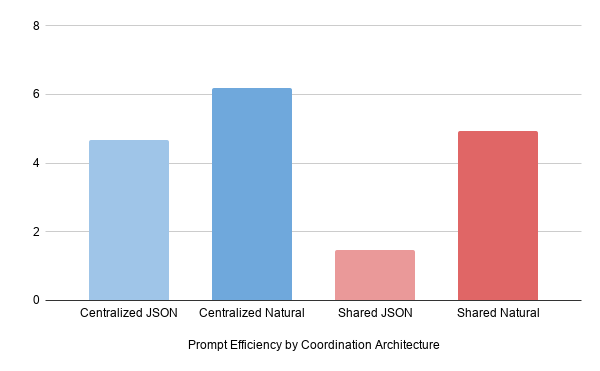
\includegraphics[width=0.82\textwidth]{figures/charts/new/prompt_efficiency_coordination_architecture.png}
\ChartPromptArchitecture
\caption{Call-normalised deliveries by prompt format within each planning architecture. Each bar is calculated from 72 matched configuration-level observations. Higher bars indicate more deliveries per 1000 model calls; the measure describes interaction frequency rather than computational cost.}
\label{fig:prompt_efficiency_coordination_architecture}
\end{figure}

These results show that the tested natural-language prompt configuration, which presented the simulator state in descriptive form, supported better collaborative task performance overall than the tested \gls{json}-based configuration. It produced higher mean deliveries and higher deliveries per 1000 model calls across all six scenario groups and for five of the six models. Phi4 showed a small \gls{json} advantage on both measures. The consistency of the broader pattern supports the answer to RQ3: at the level of the complete prompt configurations, the descriptive natural-language configuration was more effective overall, although the Phi4 result shows that the effect was model-dependent and cannot be attributed to a single formatting component.

\subsection{RQ2: Planning-Architecture Comparison}
\label{sec:results_architecture}

RQ2 compares centralized planning with shared-context per-agent planning. Because shared-context planning can call the \gls{llm} separately for multiple agents, \gls{llm} calls are partly a consequence of the architecture itself. For this reason, the architecture comparison is interpreted primarily through mean deliveries, while the call-normalised value is treated as a secondary measure of model-interaction frequency rather than computational cost.

Table~\ref{tab:central_shared_scenario} reports the scenario-level comparison, with 16 matched configuration-level observations per architecture within each scenario. Shared-context planning produced more mean deliveries in every scenario, although it also made more \gls{llm} calls. Centralized planning therefore used fewer model interactions, while shared-context planning produced higher delivery counts in this dataset.

\begin{table}[H]
\centering
\small
\resizebox{\textwidth}{!}{%
\begin{tabular}{|l|c|c|c|c|}
\hline
\textbf{Scenario} & \textbf{Central mean calls} & \textbf{Central mean del.} & \textbf{Shared mean calls} & \textbf{Shared mean del.} \\ \hline
tiny\_balanced\_1v1 & 605.31 & 3.08 & 717.89 & 6.05 \\ \hline
small\_balanced\_2v2 & 598.54 & 2.67 & 1230.46 & 4.54 \\ \hline
small\_agv\_heavy\_4v2 & 925.89 & 8.67 & 2185.60 & 13.15 \\ \hline
small\_picker\_heavy\_2v4 & 939.61 & 3.86 & 2551.91 & 8.93 \\ \hline
medium\_balanced\_4v4 & 1297.57 & 7.83 & 2412.21 & 8.18 \\ \hline
medium\_agv\_heavy\_6v2 & 816.61 & 7.69 & 1852.57 & 10.59 \\ \hline
\end{tabular}
}
\caption{Planning architecture comparison by scenario. Each architecture--scenario cell summarises 16 configuration-level observations matched by objective, prompt configuration, model, and scenario.}
\label{tab:central_shared_scenario}
\end{table}

The model-level architecture comparison uses 12 matched configuration-level observations per architecture for each model. Shared-context planning produced more mean deliveries for the Llama models, Mistral, Gemma, and Phi4, while Qwen produced more under centralized planning. The delivery gap between the two architectures generally narrowed among the larger selected models, with Qwen reversing the overall pattern. This indicates that the best planning architecture may depend on both model behaviour and scenario size.

One possible explanation for the overall shared-context advantage is that each model call selects an action for only one agent. This may reduce the number of simultaneous decisions that must be produced and avoids requiring the model to construct a mutually compatible joint action in a single response. Centralized planning nevertheless receives the complete shared state and, in principle, can account for dependencies among all agents directly. The results show that access to global information alone did not produce higher delivery performance under the centralized prompt used here; the model also had to integrate that information successfully into a joint plan.

\begin{figure}[H]
\centering
% Previous raster chart:
% 
\includegraphics[width=0.95\textwidth]{figures/charts/new/centralized_shared_deliveries_scenario.png}
\ChartArchitectureScenarios
\caption{Centralized and shared-context mean deliveries by scenario. Each bar is the mean of 16 matched configuration-level observations per architecture and scenario.}
\label{fig:centralized_shared_deliveries_scenario}
\end{figure}

\begin{figure}[H]
\centering
% Previous raster chart:
% 
\includegraphics[width=0.82\textwidth]{figures/charts/new/centralized_shared_deliveries_model.png}
\ChartArchitectureModels
\caption{Centralized and shared-context mean deliveries by model. Each bar is the mean of 12 matched configuration-level observations per architecture and model.}
\label{fig:centralized_shared_deliveries_model}
\end{figure}

Across the selected model artefacts ordered by nominal parameter size, the delivery difference between shared-context and centralized planning generally narrowed, and Qwen reversed the pattern by producing more deliveries under centralized planning. This trend is compatible with the hypothesis that some models handle the additional joint-planning demand more effectively. Related work has reported stronger performance from a larger backbone in planning-based logical reasoning~\cite{zhao2023explicitplanning}, while evaluations of autonomous language-model planning have also found substantial differences between models and identified the strongest tested model as the best performer, although its absolute success rate remained limited~\cite{valmeekam2023planning}. These findings support treating planning capability as model-dependent, but they do not establish parameter count as the cause of the present architecture differences because the evaluated models also differ in model family and post-training. Across the full architecture comparison, shared-context planning produced higher mean deliveries in all six scenario groups and for five of the six selected models. The consistency across different layouts, agent populations, and role balances indicates that this advantage was not restricted to one type of collaboration demand. RQ2 therefore reveals a trade-off: shared-context planning generally produced higher delivery performance in the tested setting, whereas centralized planning required fewer model interactions; the narrowing model-level gap and Qwen reversal show that the preferred architecture remains model-dependent.

\subsection{RQ1: Model Choice and Scenario Complexity}
\label{sec:results_model_choice}

RQ1 asks how grounded collaborative task performance varies among the selected locally deployable models spanning different nominal parameter sizes. The model-level evidence is considered across the prompt-configuration comparison in Table~\ref{tab:json_natural_model} and Figure~\ref{fig:prompt_efficiency_models}, the architecture comparison in Figure~\ref{fig:centralized_shared_deliveries_model}, and the broader matched comparison in Figure~\ref{fig:model_matched_performance}.

For the broader comparison, a configuration is included only when all six models have observations for the same objective, planning architecture, prompt configuration, and scenario. This gives 48 configuration-level observations per model, divided equally between 24 natural-language and 24 \gls{json} configurations. The same configurations and prompt-format balance are therefore represented for every model in Figure~\ref{fig:model_matched_performance}.

\begin{figure}[H]
\centering
\ChartMatchedModels
\caption{Delivery performance across the matched model comparison. Each model uses the same 48 objective--architecture--prompt--scenario configurations, comprising 24 natural-language and 24 \gls{json} configurations. The second measure reports deliveries per 1000 model calls.}
\label{fig:model_matched_performance}
\end{figure}

Figure~\ref{fig:model_matched_performance} shows that llama 3b achieved the highest mean delivery count, at 7.21, while Phi4 achieved the highest call-normalised value, at 7.86 deliveries per 1000 calls. Llama 1b produced the lowest values on both measures. Mistral, Gemma, and Qwen achieved similar mean delivery counts, but their call-normalised values differed.

The prompt-configuration comparison provides a second model-level view. Table~\ref{tab:json_natural_model} and Figure~\ref{fig:prompt_efficiency_models} show higher natural-language mean deliveries and call-normalised values for five models; Phi4 instead produced slightly higher values under \gls{json} on both measures. The size of the prompt-related difference also varied substantially by model. Llama 3b achieved the highest natural-language mean delivery count, while Phi4 achieved the highest natural-language call-normalised value in the updated matched subset. The architecture comparison in Figure~\ref{fig:centralized_shared_deliveries_model} also shows a model-dependent pattern: shared-context planning produced more deliveries for five models, whereas Qwen produced more under centralized planning. Model performance therefore changed with both prompt configuration and planning architecture.

Scenario complexity also affected performance. Natural-language prompts produced the highest call-normalised delivery values in the tiny balanced and small AGV-heavy scenarios, with a similarly high value in the medium AGV-heavy scenario, while the values were lower in the small picker-heavy and small balanced scenarios. This suggests that model performance is shaped by the interaction between model behaviour, prompt representation, planning architecture, and the collaboration demands of the scenario.

The comparatively low performance of some larger models should not be interpreted as evidence that larger models are intrinsically less suitable for collaborative planning. Rather, the results show that, for some of the evaluated configurations, smaller models achieved task performance comparable to or better than that of larger models. Since smaller models generally require less memory and inference computation, they may provide a favourable performance--resource trade-off for locally deployed planners~\cite{dawane2026onddeviceslm}. Computational cost was not measured directly in this comparison, so the present result establishes competitive task performance rather than a quantified cost reduction. It nevertheless indicates that increasing nominal parameter count is not always necessary to obtain effective performance in a fixed collaborative planning setting.

Overall, the results answer RQ1 at the level of the selected model artefacts: model choice mattered, but performance did not increase consistently with nominal parameter size. Llama 3b produced the highest mean delivery count in the balanced 48-configuration comparison, while Phi4 produced the highest call-normalised value. Larger models such as Gemma 12b and Qwen 14b did not uniformly dominate these measures. Since all six models were compared over the same 24 natural-language and 24 \gls{json} configurations, these changing rankings support the conclusion that nominal parameter size alone did not predict collaborative task performance among the selected model artefacts.

\subsection{Model Adaptability to Objectives}
\label{sec:results_objective_sensitivity}

This analysis compares three objective families: reducing \gls{llm} calls, balancing shelf delivery with battery awareness, and prioritising battery management to examine how model behaviour changed with the stated objective.

Table~\ref{tab:objective_shared_natural} summarises the aggregate objective-level results for 72 matched configurations per objective. Battery produced the lowest mean number of calls, while Battery + Shelf produced the highest mean deliveries and call-normalised delivery value. Calls produced slightly fewer calls than Battery + Shelf, but also fewer deliveries and a lower call-normalised value.

\begin{table}[H]
\centering
\small
\resizebox{\textwidth}{!}{%
\begin{tabular}{|l|c|c|c|c|}
\hline
\textbf{Objective} & \textbf{Matched combinations} & \textbf{Mean calls} & \textbf{Mean deliveries} & \textbf{Deliveries/1000 calls} \\ \hline
Calls & 72 & 1267.54 & 6.82 & 5.38 \\ \hline
Battery + Shelf & 72 & 1272.45 & 7.48 & 5.88 \\ \hline
Battery & 72 & 1241.86 & 6.51 & 5.24 \\ \hline
\end{tabular}
}
\caption{Objective-level calls and deliveries across configurations matched among the Calls, Battery + Shelf, and Battery objectives.}
\label{tab:objective_shared_natural}
\end{table}

To examine whether models adapted to the call-reduction objective, the analysis compares each model under the matched Calls and Battery + Shelf configurations. The mean-call difference in Figure~\ref{fig:model_call_reduction_adaptability} is computed as Calls minus Battery + Shelf, so negative values indicate fewer calls under the Calls objective. Llama 1b, llama 3b, Phi4, and Qwen produced fewer calls under Calls, whereas Mistral and Gemma produced more. The response to the call-reduction objective was therefore model-dependent rather than consistent across all models.

Battery-related behaviour was examined using the descriptive battery-aware productivity score defined in Eq.~\ref{eq:battery-aware-productivity}. The score indicates whether charging-station occupancy occurred together with successful delivery performance; it does not distinguish necessary from unnecessary charging and is not an optimality measure. Table~\ref{tab:battery_aware_productivity} reports this score across the matched three-objective configurations. The Battery objective produced the highest score for llama 1b and Mistral, Battery + Shelf produced the highest score for llama 3b, Phi4, and Qwen, and Calls produced the highest score for Gemma. The differing rankings show that the Battery objective did not produce a consistent improvement across the evaluated models.

\begin{table}[H]
\centering
\small
\begin{tabular}{|l|c|c|c|}
\hline
\textbf{Model} & \textbf{Calls score} & \textbf{Battery + Shelf score} & \textbf{Battery score} \\ \hline
llama 1b (3.2) & 41.44 & 48.76 & 51.54 \\ \hline
llama 3b (3.2) & 135.36 & 214.35 & 207.94 \\ \hline
mistral 7b & 98.65 & 153.43 & 166.25 \\ \hline
gemma 12b & 106.92 & 84.98 & 58.05 \\ \hline
phi4 & 50.14 & 76.99 & 15.83 \\ \hline
qwen 14b (2.5) & 95.19 & 104.79 & 100.24 \\ \hline
\end{tabular}
\caption{Battery-aware productivity by model and objective, using the descriptive score defined in Eq.~\ref{eq:battery-aware-productivity}. Each model--objective cell uses $n=12$ matched configuration-level observations.}
\label{tab:battery_aware_productivity}
\end{table}

A direct battery-outcome comparison was made across 72 matched natural-language configurations per objective. The Battery objective produced a higher mean minimum battery and slightly lower zero-battery fractions. Its below-threshold fraction was slightly higher, while mean deliveries and charging-station utilisation were lower.

For each configuration, the minimum battery is the lowest value reached by any agent during the run. The agent-step fraction is the proportion of all agent-step observations below the critical threshold of 30. The agent-zero fraction is the proportion of agents that reached zero battery, and the run-zero fraction is the proportion of configurations in which at least one agent reached zero. The table reports the mean of each measure across the matched configurations.

\begin{table}[H]
\centering
\small
\resizebox{\textwidth}{!}{%
\begin{tabular}{|l|c|c|c|c|c|c|c|}
\hline
\textbf{Objective} & \textbf{Matched} & \textbf{Mean del.} & \textbf{Charger util. (\%)} & \textbf{Mean min. battery} & \textbf{Agent-step frac. $<30$} & \textbf{Agent-zero frac.} & \textbf{Run-zero frac.} \\ \hline
Battery & 72 & 6.66 & 13.91 & 5.01 & 0.292 & 0.442 & 0.736 \\ \hline
Battery + Shelf & 72 & 7.26 & 14.87 & 3.70 & 0.286 & 0.475 & 0.750 \\ \hline
Battery $-$ Battery + Shelf & --- & $-0.60$ & $-0.95$ & $+1.31$ & $+0.006$ & $-0.033$ & $-0.014$ \\ \hline
\end{tabular}
}
\caption{Direct battery outcomes across matched Battery and Battery + Shelf configurations. Repeated runs are averaged before each configuration receives equal weight.}
\label{tab:direct_battery_outcomes}
\end{table}

\begin{figure}[H]
\centering
% Previous raster chart:
% 
\includegraphics[width=0.82\textwidth]{figures/charts/new/model_adaptability_call_reduction.png}
\ChartCallAdaptability
\caption{Model response to the \gls{llm} call-reduction objective. Mean-call difference is computed as Calls minus Battery + Shelf; negative values indicate fewer calls under Calls. Each model--objective mean uses $n=24$ matched configuration-level observations.}
\label{fig:model_call_reduction_adaptability}
\end{figure}

\begin{figure}[H]
\centering
% Previous raster chart:
% 
\includegraphics[width=0.82\textwidth]{figures/charts/new/battery_aware_productivity_objectives.png}
\ChartBatteryProductivity
\caption{Battery-aware productivity across objective prompts. Higher bars indicate that charging utilisation occurred together with more deliveries; the score is descriptive rather than an optimality measure. Each bar uses $n=12$ matched configuration-level observations.}
\label{fig:battery_aware_productivity}
\end{figure}

The objective changes produced mixed, model-dependent responses. Under the Calls objective, four models reduced their mean number of calls, while Mistral and Gemma increased it. Across the matched pairwise comparison, the aggregate reduction relative to Battery + Shelf was small, and Battery produced the lowest mean call count in the three-objective comparison. The Calls instruction therefore affected the models differently but did not consistently achieve its stated purpose. For the Battery objective, the mean minimum battery increased by 1.31 and the agent-zero and run-zero fractions decreased slightly, but the below-threshold fraction increased by 0.006 and mean deliveries decreased by 0.60. These opposing results suggest a small change in battery-related behaviour rather than a general improvement in battery management. Since the model weights and controller were unchanged between the matched objective configurations, the observed differences support sensitivity to the stated objective, but not consistent adaptation to the requested objectives.

\subsection{Summary of Findings}

The main research question is answered positively within the tested simulator: prompted \glspl{llm} can support grounded high-level decision-making for heterogeneous robot collaboration. Successful shelf deliveries were observed across the evaluated models, architectures, prompt configurations, and scenarios. This finding supports the answer because it shows that the generated decisions could be validated, executed, and used to complete collaborative tasks. It establishes feasibility within Battery-TA-RWARE, but not superiority over non-LM planning methods.

For RQ1, the selected model affected collaborative task performance, but nominal parameter size alone did not predict performance. Llama 3b achieved the highest mean delivery count and Phi4 the highest call-normalised value in the matched 48-configuration comparison, while the larger Gemma and Qwen models did not consistently dominate. This finding supports the answer because all models were evaluated over the same balanced set of 24 natural-language and 24 \gls{json} configurations, yet their performance did not increase with parameter size.

For RQ2, shared-context planning generally produced higher delivery performance, while centralized planning required fewer model interactions. Shared-context planning produced higher mean deliveries in all six scenario groups and for five of the six models. Across the selected model artefacts ordered by nominal parameter size, the delivery difference between the architectures generally narrowed, with Qwen eventually producing more deliveries under centralized planning. This finding supports the answer because the shared-context advantage appeared across every scenario group, while the narrowing model-level difference and Qwen reversal show that the architecture effect remains model-dependent. Since the models belong to different families, the trend does not establish parameter size as its cause.

For RQ3, the complete natural-language prompt configuration was more effective overall than the complete \gls{json}-based configuration. Natural language produced higher mean deliveries and call-normalised values in all six scenario groups and for five of the six models; Phi4 showed a small \gls{json} advantage on both measures. This finding supports the answer because the same overall pattern appears in the scenario-level and most model-level matched comparisons. The result applies to the complete prompt configurations and does not isolate the input representation from the output constraints.

The supplementary objective-sensitivity analysis did not show consistent adaptation. The call-reduction objective did not consistently reduce \gls{llm} usage, and the direct battery indicators showed only small, mixed differences between the Battery and Battery + Shelf objectives. These findings support only limited objective sensitivity and do not provide conclusive evidence of adaptation.


\section{Conclusions and Future Work}
\label{sec:conclusions}
This thesis evaluates \gls{llm}-driven decision-making for heterogeneous multi-robot collaboration in a task-assignment warehouse setting with battery constraints.
The implemented control loop grounds decisions to discrete environment action identifiers, queries an \gls{llm} using centralized or per-agent shared-context prompts, and enforces feasibility through action-mask validation.

The reported comparisons use matched configuration-level observations drawn from the call-aware, battery-plus-shelf, and battery-aware objective families. Prompt-configuration, planning-architecture, and objective-sensitivity results include only configurations with the required counterpart, and repeated executions with the same configuration identifiers are averaged before comparison.

The experiments answer the main research question by showing that prompted \glspl{llm} can produce grounded high-level decisions and complete collaborative shelf deliveries within the tested simulator framework. The occurrence of successful deliveries across models, architectures, prompt configurations, and scenarios supports the conclusion that this approach is feasible within the tested setting, while the absence of a non-LM baseline prevents a claim of superiority over other planning methods. For RQ1, collaborative task performance across the selected model artefacts did not increase consistently with nominal parameter size in the balanced 24-natural and 24-\gls{json} comparison. For RQ2, shared-context planning produced higher mean deliveries in all six scenario groups and for five of the six selected models, while centralized planning used fewer \gls{llm} calls. For RQ3, the tested natural-language prompt configuration produced higher mean deliveries and call-normalised delivery values across all six scenario groups and for five of the six models; Phi4 showed a small \gls{json} advantage on both measures. The objective-sensitivity analysis showed mixed adaptation: the call-aware objective did not consistently reduce \gls{llm} usage, and the direct battery indicators showed small, mixed differences between the Battery and Battery + Shelf objectives.

\subsection{Future Work}
\label{sec:futurework}
The capabilities of language models and the systems built around them are developing rapidly. Consequently, the results in this thesis represent one set of models and configurations at a particular point in time, rather than a final assessment of language-model-based robot collaboration. Model choice, decoding parameters, prompt design, context construction, and tool access can all affect the resulting behaviour. Future evaluations should therefore treat these choices as experimental variables and document them sufficiently to distinguish improvements in the underlying model from improvements in the surrounding system.

One direction is to extend the planner with retrieval-augmented generation and external tools exposed through Model Context Protocol servers. Retrieval could provide task-relevant information without placing all available knowledge in every prompt, while reusable skills could define how the model accesses simulator state, robot capabilities, operational rules, or previous experience. Such additions should be evaluated separately from the base model because they alter the information and actions available to the planner. Of particular interest is whether they improve grounded decision-making and generalisation to new warehouse configurations, rather than only increasing system complexity.

The shared-context architecture studied here gives each agent access to a common state description, but it does not investigate communication as a behaviour in its own right. A further study could allow agents to communicate their local state, intended action, or request for assistance directly to one another. With a retained communication history or an explicit adaptation mechanism, repeated interactions could then be examined to determine whether the agents converge towards a useful communication protocol: what information is sent, when communication occurs, and which agents need to receive it. Comparing unrestricted communication with bandwidth-, latency-, or cost-constrained communication would help establish whether the exchanged messages contribute to collaboration or merely duplicate information already available in the environment state.

Deployment-oriented model optimisation is another open direction. Tools such as Embedl\footnote{\url{https://www.embedl.com/}},
which target the optimisation of models for specific hardware platforms,
may reduce latency, memory use, or energy consumption and thereby make local inference more practical. However, techniques used to obtain these gains may also change model behaviour. It would therefore be useful to evaluate the unmodified and optimised versions of a model on the same scenarios, measuring not only execution performance but also action validity, planning quality, robustness, and collaborative task performance. This would reveal whether hardware-specific optimisation introduces a capability loss that is relevant to robot decision-making~\cite{dawane2026onddeviceslm}.

The experiments reported in this thesis were executed on an NVIDIA RTX A4000. Repeating the same protocol on other GPU generations, accelerator architectures, and resource-constrained edge hardware would test the portability of the findings. The comparison should keep the model artifact, inference configuration, and simulator conditions fixed where possible, while recording differences in numerical precision, runtime, memory use, and energy consumption. This would help determine whether the observed performance trends are stable across hardware or partly dependent on the inference stack used in the present study.

Finally, the limited number of completed runs and simulator initialisations restricts the statistical confidence of the present analysis. Future experiments should use more runs, multiple independently selected seeds, and balanced coverage of every model--scenario--configuration combination. Reporting uncertainty intervals and sensitivity across seeds would make it possible to distinguish persistent trends from variation caused by initial conditions or stochastic generation. Useful extensions would also include stricter structured-output validation, comparison with multi-agent reinforcement-learning baselines, and a joint analysis of task performance, inference latency, token usage, and energy cost.



%%%% References
\newpage

% Use one of these (paths included so BibTeX finds the .bst files in this repo):
%   IEEEtranS gives numbered references like [42] sorted by author,
%   IEEEtranSA gives ``alpha''-style references like [Lam81] (also sorted by author)
\bibliographystyle{./IEEEtran/bibtex/IEEEtranS}
%\bibliographystyle{./IEEEtran/bibtex/IEEEtranSA}

% Here comes the bibliography/references.
% För att göra inställningar för IEEEtranS/SA kan man använda ett speciellt bibtex-entry @IEEEtranBSTCTL,
% se IEEEtran/bibtex/IEEEtran_bst_HOWTO.pdf, avsnitt VII, eller sista biten av IEEEtran/bibtex/IEEEexample.bib.
\bibliography{./dependencies/bibconfig,refs.bib}
%\bibliography{refs.bib}

\newpage

%%%% Appendix

\appendix 
\section{Appendix}
\label{app:appendix}

\subsection{Reproducibility: Experiment Runners}
\label{app:repro}
The reported experiments are executed from the Battery-TA-RWARE repository using the objective-family runners for centralized and shared-context planning.
Earlier exploratory scripts are not part of the reported comparison.
The examples below show the command structure used by the current protocol; the seed, prompt format, model subset, and result directory can be changed for a particular session.

\begin{lstlisting}[caption=Run Objective 1 with the shared-context planner., label=listing:run_obj1_shared]
python Battery-TA-RWARE/scripts/run_obj1_shared_context_llm.py \
  --prompt_format language \
  --max_steps 0 \
  --max_busy_steps_for_replan 10 \
  --max_inactivity_steps 500 \
  --disable_support_needed_soon \
  --find_path_agent_aware_always \
  --seed 0
\end{lstlisting}

\begin{lstlisting}[caption=Run Objective 1 with the centralized planner., label=listing:run_obj1_centralized]
python Battery-TA-RWARE/scripts/run_obj1_centralized_llm.py \
  --prompt_format language \
  --max_steps 0 \
  --max_busy_steps_for_replan 10 \
  --max_inactivity_steps 500 \
  --disable_support_needed_soon \
  --find_path_agent_aware_always \
  --seed 0
\end{lstlisting}

\begin{lstlisting}[caption=Run Objective 2 with the shared-context planner., label=listing:run_obj2_shared]
python Battery-TA-RWARE/scripts/run_obj2_shared_context_llm.py \
  --prompt_format language \
  --max_steps 0 \
  --max_busy_steps_for_replan 10 \
  --max_inactivity_steps 500 \
  --disable_support_needed_soon \
  --find_path_agent_aware_always \
  --seed 0
\end{lstlisting}

\begin{lstlisting}[caption=Run Objective 2 with the centralized planner., label=listing:run_obj2_centralized]
python Battery-TA-RWARE/scripts/run_obj2_centralized_llm.py \
  --prompt_format language \
  --max_steps 0 \
  --max_busy_steps_for_replan 10 \
  --max_inactivity_steps 500 \
  --disable_support_needed_soon \
  --find_path_agent_aware_always \
  --seed 0
\end{lstlisting}

\begin{lstlisting}[caption=Run Objective 3 with the shared-context planner., label=listing:run_obj3_shared]
python Battery-TA-RWARE/scripts/run_obj3_shared_context_llm.py \
  --prompt_format language \
  --max_steps 0 \
  --max_busy_steps_for_replan 10 \
  --max_inactivity_steps 500 \
  --disable_support_needed_soon \
  --find_path_agent_aware_always \
  --seed 0
\end{lstlisting}

\begin{lstlisting}[caption=Run Objective 3 with the centralized planner., label=listing:run_obj3_centralized]
python Battery-TA-RWARE/scripts/run_obj3_centralized_llm.py \
  --prompt_format language \
  --max_steps 0 \
  --max_busy_steps_for_replan 10 \
  --max_inactivity_steps 500 \
  --disable_support_needed_soon \
  --find_path_agent_aware_always \
  --seed 0
\end{lstlisting}

The same commands can be run with \nolinkurl{--prompt_format json} to execute the structured prompt variant.
Objective 1 also supports \nolinkurl{--selected_models}.
For Objectives 2 and 3, the corresponding single-model filter is \nolinkurl{--only_model}.
The seed is logged for traceability.

\subsection{Result Directories}
\label{app:result_dirs}
The objective-family runners write session outputs under the following default directories:
\begin{itemize}
    \item \nolinkurl{results/obj1_shared_context_llm_experiments}
    \item \nolinkurl{results/obj1_centralized_llm_experiments}
    \item \nolinkurl{results/obj2_shared_context_llm_experiments}
    \item \nolinkurl{results/obj2_centralized_llm_experiments}
    \item \nolinkurl{results/obj3_shared_context_llm_experiments}
    \item \nolinkurl{results/obj3_centralized_llm_experiments}
\end{itemize}
These raw step-level result directories are retained separately because their size is unsuitable for the source repository; the repository contains the experiment implementation and runner commands.
Each session stores aggregate summaries together with per-run JSON summaries and detailed logs.
The aggregate analysis uses the retained runs from these outputs and follows the protocol described in Section~\ref{sec:method_scenarios_models_metrics}.

\subsection{Prompt Excerpt}
\label{app:prompt_excerpt}
The full prompts are generated programmatically from the simulator state.
The excerpt below is illustrative and shows the action-id grounding and output contract used by the natural-language shared-context prompt.

\begin{lstlisting}[caption=Illustrative shared-context natural-language prompt excerpt., label=listing:prompt_excerpt]
Objective:
Maximize useful warehouse progress under the current objective.

Current agent:
agent_0, role=AGV, position=(8, 3), battery=72, carrying=None

Shared context:
- Requested shelf 24 is at position (11, 5), action id 50.
- Picker support is required at shelf action id 50.
- Charging station action id 7 is currently unoccupied.

Candidate actions:
- action=0, type=NOOP, distance=0, instruction=wait only if blocked
- action=50, type=SHELF, distance=8, instruction=go to requested shelf
- action=7, type=CHARGING, distance=11, instruction=use if battery is unsafe

Output contract:
Return only:
Action: <integer action id>
Steps: <integer hold duration>
Reason: <short reason>
\end{lstlisting}

For the centralized planner, the prompt contains the shared warehouse context plus one planning block for each agent being replanned.
The centralized response must contain one action for each listed agent.
For the JSON prompt variant, the same information is represented as a structured object and the model is constrained to return a machine-readable action object or action list.

\subsection{Run Summary Fields}
\label{app:run_summary_fields}
The aggregate CSV files use the following run-level fields:
\begin{lstlisting}[caption=Run-summary CSV fields used for aggregation., label=listing:summary_fields]
Objective
Arch
Prompt
Model
Scenario
Seed
Run
llm_calls
json_generation_failures
llm_missing_or_invalid_actions
charging_station_utilization_rate
elapsed_seconds
steps to first delivery
total deliveries
total steps
deliveries_per_1000_steps
llm_calls_per_1000_steps
llm_calls_per_delivery
invalid_action_rate
json_failure_rate
summary_json_path
\end{lstlisting}

The main analysis uses total deliveries, \gls{llm} calls, deliveries per 1000 \gls{llm} calls, and the descriptive battery-aware productivity score defined in Section~\ref{sec:method_scenarios_models_metrics}.
The remaining fields are retained for filtering, traceability, and diagnostic interpretation.
Parsing and invalid-action fields support diagnostic tracing of malformed outputs and configuration errors.
The \nolinkurl{summary_json_path} field links each aggregate row to the corresponding detailed run summary.


\end{document}
